% Created 2021-11-01 Mon 16:14
\documentclass[9pt, b5paaper]{book}
\usepackage[UTF8]{ctex}
\usepackage{xltxtra}
\usepackage{bera}
\usepackage[T1]{fontenc}
\usepackage[scaled]{beraserif}
\usepackage[scaled]{berasans}
\usepackage[scaled]{beramono}
\usepackage{graphicx}
\usepackage{xcolor}
\usepackage{multirow}
\usepackage{multicol}
\usepackage{float}
\usepackage{textcomp}
\usepackage{geometry}
\geometry{left=1.2cm,right=1.2cm,top=1.5cm,bottom=1.2cm}
\usepackage{algorithm}
\usepackage{algorithmic}
\usepackage{latexsym}
\usepackage{natbib}
\usepackage{minted}
\newminted{common-lisp}{fontsize=ootnotesize}
\usepackage[xetex,colorlinks=true,CJKbookmarks=true,linkcolor=blue,urlcolor=blue,menucolor=blue]{hyperref}
\date{\today}
\title{dp}
\hypersetup{
  pdfkeywords={},
  pdfsubject={},
  pdfcreator={Emacs 27.1 (Org mode 8.2.7c)}}
\begin{document}

\maketitle
\tableofcontents


\chapter{Dynamic Programming, 动态规划}
\label{sec-1}
\section{总结}
\label{sec-1-1}
\begin{itemize}
\item 根据CLRS,动态规划分为两种:
\item top-down with memoization (递归记忆化搜索)
\end{itemize}
等价于带缓存的,搜索树上的 DFS
比较贴近于新问题正常的思考习惯
\begin{itemize}
\item bottom-up (自底向上循环迭代)
\end{itemize}
以 "reverse topological order" 处理
每个子问题下面依赖的所有子问题都算完了才开始计算当前
一般依赖于子问题之间天然的 "size

\section{198. House Robber - Medium}
\label{sec-1-2}
You are a professional robber planning to rob houses along a street. Each house has a certain amount of money stashed, the only constraint stopping you from robbing each of them is that adjacent houses have security systems connected and it will automatically contact the police if two adjacent houses were broken into on the same night.

Given an integer array nums representing the amount of money of each house, return the maximum amount of money you can rob tonight without alerting the police.
\subsection{解题思路与分析}
\label{sec-1-2-1}
\begin{itemize}
\item 对于每一个住户来说,只有两种选择:
\begin{itemize}
\item 偷这一户人家的,下一家不要
\item 不偷这一家的,去偷下一家的
\end{itemize}
\end{itemize}
\begin{minted}[frame=lines,fontsize=\scriptsize,linenos=false]{java}
private int dfs(int [] arr, int idx) {
    if (idx >= n) return 0;
    if (dp[idx] > 0) return dp[idx];
    return dp[idx] = Math.max(dfs(arr, idx+2) + arr[idx], dfs(arr, idx+1)); // 不要忘记记忆——记住答案!!!
}
int [] dp;
int n;
public int rob(int[] a) {
    if (Arrays.stream(a).sum() == 0) return 0;
     n = a.length;
     dp = new int [n];
     return dfs(a, 0);
}
\end{minted}
\section{213. House Robber II}
\label{sec-1-3}
You are a professional robber planning to rob houses along a street. Each house has a certain amount of money stashed. All houses at this place are arranged in a circle. That means the first house is the neighbor of the last one. Meanwhile, adjacent houses have a security system connected, and it will automatically contact the police if two adjacent houses were broken into on the same night.
Given an integer array nums representing the amount of money of each house, return the maximum amount of money you can rob tonight without alerting the police.
\subsection{解题思路与分析}
\label{sec-1-3-1}
\begin{itemize}
\item 与上一题不同的是:因为是环形数组,数组首尾相连,相邻的两户人家只能偷一家
\item 问题就转化成了:我要么去偷[0, n-2]这些人家的,要么去偷[1, n-1]这些人家的,包括首尾
\item 这成了上一题的稍微变形与套娃
\end{itemize}
\begin{minted}[frame=lines,fontsize=\scriptsize,linenos=false]{java}
private int dfs(int [] arr, int i, int j, int idx) {
    if (idx > j) return 0;
    if (dp[idx] != -1) return dp[idx];
    return dp[idx] = Math.max(dfs(arr, i, j, idx+2) + arr[idx], dfs(arr, i, j, idx+1));
}
int [] dp;
int n;
public int rob(int[] arr) {
     n = arr.length;
     if (n == 1) return arr[0];
     dp = new int [n];
     Arrays.fill(dp, -1);
     int max = dfs(arr, 1, n-1, 1);
     Arrays.fill(dp, -1); // 不要忘了dp数组的重置与重新计算
     // return Math.max(dfs(arr, 1, n-1, 1), dfs(arr, 0, n-2, 0)); // BUG: 因为dp数组不重置,会发生数据混淆,得到错误答案
     return Math.max(max, dfs(arr, 0, n-2, 0));
}
\end{minted}
\section{740. Delete and Earn: 一类题目,变形了你还认得出来吗?}
\label{sec-1-4}
You are given an integer array nums. You want to maximize the number of points you get by performing the following operation any number of times:
Pick any nums[i] and delete it to earn nums[i] points. Afterwards, you must delete every element equal to nums[i] - 1 and every element equal to nums[i] + 1.
Return the maximum number of points you can earn by applying the above operation some number of times.
\subsection{解题思路与分析}
\label{sec-1-4-1}
\begin{itemize}
\item 关键题意理解:对于nums = [2, 2, 3, 3, 3, 4],如果我们选了数字3,则要删除每一个(所有)2和4,之后数组变为[3, 3],此时如果再选3,并不会删除其他元素,剩余数组变为\footnote{DEFINITION NOT FOUND.},再选3,数组变为空,返回结果是3+3+3=9。
\item 将上面的例子转化为House Robber的形式,nums' = [0, 0, 22, 33, 4],nums'[i]代表值为i的数字的总数和(或者数字(下标)i在原数组中出现的次数),每次若选择nums'数组的一个元素,则相邻元素不能在下一次被选中(包括其所有的重复计数),相当于被全部删去。转化后,用House Robber的思路来处理nums'数组即可。
\end{itemize}
\begin{minted}[frame=lines,fontsize=\scriptsize,linenos=false]{java}
private int dfs(int [] cnt, int i) {
    if (i >= N) return 0;
    if (dp[i] > 0) return dp[i];
    return dp[i] = Math.max(dfs(cnt, i+2) + cnt[i]*i, dfs(cnt, i+1));
}
int [] dp;
int N;
public int deleteAndEarn(int[] nums) {
    int n = nums.length, max = Arrays.stream(nums).max().getAsInt();
    N = max+1;
    int [] cnt = new int [N];
    for (Integer v : nums) 
        cnt[v]++;
    dp = new int [N];
    int i = 0;
    while (i < N && cnt[i] == 0) i++;
    return dfs(cnt, i);
}
\end{minted}
\begin{itemize}
\item dp解
\end{itemize}
\begin{minted}[frame=lines,fontsize=\scriptsize,linenos=false]{java}
public int deleteAndEarn(int[] nums) {
    int n = nums.length, N = 10001;
    int [] cnt = new int [N];
    for (Integer v : nums) 
        cnt[v] += v;
    int preOne = 0, preTwo = 0, ans = 0; // 相当于是滚动数组,把一维dp压缩为两个位置
    for (Integer v : cnt) {
        ans = Math.max(preOne, v + preTwo);
        preTwo = preOne;
        preOne = ans;
    }
    return ans;
}
\end{minted}


\section{2019. The Score of Students Solving Math Expression - Hard 有人说这是区间dp,无感}
\label{sec-1-5}
You are given a string s that contains digits 0-9, addition symbols '+', and multiplication symbols '*' only, representing a valid math expression of single digit numbers (e.g., 3+5*2). This expression was given to n elementary school students. The students were instructed to get the answer of the expression by following this order of operations:

Compute multiplication, reading from left to right; Then,
Compute addition, reading from left to right.
You are given an integer array answers of length n, which are the submitted answers of the students in no particular order. You are asked to grade the answers, by following these rules:

If an answer equals the correct answer of the expression, this student will be rewarded 5 points;
Otherwise, if the answer could be interpreted as if the student applied the operators in the wrong order but had correct arithmetic, this student will be rewarded 2 points;
Otherwise, this student will be rewarded 0 points.
Return the sum of the points of the students.
\subsection{解题思路与分析}
\label{sec-1-5-1}
\begin{itemize}
\item 思路是记忆化搜索。先求一下正确答案,然后开始算所有可能得到的错误答案。枚举运算符,然后递归求解两边可能的答案,汇总成当前表达式可能得到的答案。用记忆化的方式避免重复计算。
\item 时间复杂度O(l$_{\text{s}}^{\text{3}}$+l$_{\text{A}}$)),空间O(l$_{\text{s}}^{\text{2}}$)。注意有1000这个限制,上面所说的复杂度的常数是1000$^{\text{2,是很大的}}$
\end{itemize}

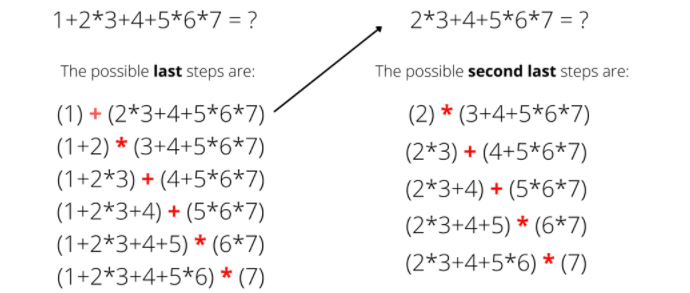
\includegraphics[width=.9\linewidth]{./pic/score.png}

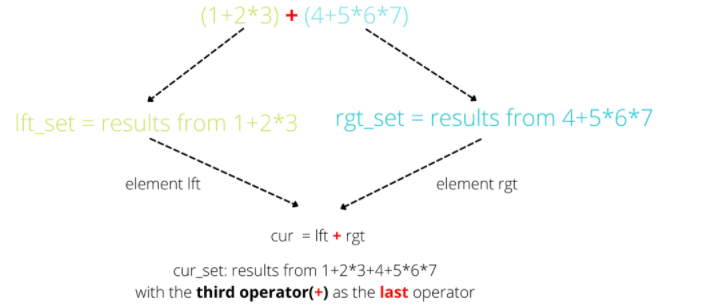
\includegraphics[width=.9\linewidth]{./pic/score2.png}

\begin{minted}[frame=lines,fontsize=\scriptsize,linenos=false]{java}
private int compute(String t) {
    ArrayDeque<Integer> st = new ArrayDeque<>();
    char [] s = t.toCharArray();
    for (int i = 0; i < s.length; i++) {
        char c = s[i];
        if (Character.isDigit(c)) 
            if (i > 0 && s[i-1] == '*') 
                st.push(st.pop() * (c-'0'));
            else st.push(c-'0');
    }
    int ans = 0;
    while (!st.isEmpty()) 
        ans += st.pop();
    return ans;
}
Set<Integer> dfs(String t, int l, int r, Set<Integer> [][] f) {
    if (f[l][r] != null) return f[l][r]; // 有记忆则调取记忆
    char [] s = t.toCharArray();
    int n = t.length(), v = 0;
    f[l][r] = new HashSet<>();
    if (l == r) {
        f[l][r].add(s[l] - '0');
        return f[l][r];
    }
    for (int i = l+1; i < r; i++) 
        if (!Character.isDigit(s[i])) { // 递归求解左右两边可能算出的答案
            Set<Integer> left = dfs(t, l, i-1, f);
            Set<Integer> right = dfs(t, i+1, r, f);
            for (Integer va : left) 
                for (Integer vb : right) {
                    if (s[i] == '*') v = va * vb;
                    else v = va + vb;
                    if (v >= 0 && v <= 1000) f[l][r].add(v);
                }
        }
    return f[l][r];
}
public int scoreOfStudents(String s, int [] num) { 
    int m = num.length, res = compute(s), n = s.length(), ans = 0;
    Set<Integer> [][] f = new HashSet[n][n]; // 第一次见,学习一下
    dfs(s, 0, n-1, f);
    Set<Integer> can = f[0][n-1];        // candidates: of wrong answers
    for (Integer v : num) 
        if (v == res) ans += 5;
        else if (can.contains(v)) ans += 2;
    return ans;
}
\end{minted}

\section{312. Burst Balloons 区间型动态规划的典型代表}
\label{sec-1-6}
You are given n balloons, indexed from 0 to n - 1. Each balloon is painted with a number on it represented by an array nums. You are asked to burst all the balloons.
If you burst the ith balloon, you will get nums[i - 1] * nums[i] * nums[i + 1] coins. If i - 1 or i + 1 goes out of bounds of the array, then treat it as if there is a balloon with a 1 painted on it.
Return the maximum coins you can collect by bursting the balloons wisely.
\begin{minted}[frame=lines,fontsize=\scriptsize,linenos=false]{java}
public int maxCoins(int[] nums) {
    int n = nums.length;
    int [][]  dp = new int [n+2][n+2];
    int [] arr = new int [n+2];
    System.arraycopy(nums, 0, arr, 1, n);
    arr[0] = arr[n+1] = 1;  // [0, n+1] ==> [1, n]
    int j = 0;
    for (int len = 1; len <= n; len++) { // [1, n]
        for (int i = 1; i+len-1 <= n; i++) { // [1, n]
            j = i + len - 1;
            for (int k = i; k <= j; k++) 
                dp[i][j] = Math.max(dp[i][j], dp[i][k-1] + dp[k+1][j] + arr[i-1]*arr[k]*arr[j+1]);
        }
    }
    return dp[1][n];
}
// 0    0    0    0    0    0
// 0    3    30   159  167  0
// 0    0    15   135  159  0
// 0    0    0    40   48   0
// 0    0    0    0    40   0
// 0    0    0    0    0    0
private int memorizedSearch(int [] arr, int x, int y) {
    if (dp[x][y] > 0) return dp[x][y];
    // if (x == y) return dp[x][y] = arr[x]; // 没有这些个边际条件
    // if (x == y-1) 
    //     return dp[x][y] = arr[x] * arr[y] + Math.max(arr[x], arr[y]);
    int max = 0;
    for (int i = x; i <= y; i++) {
        max = Math.max(max, memorizedSearch(arr, x, i-1) + memorizedSearch(arr, i+1, y) + arr[x-1]*arr[i]*arr[y+1]);
    }
    return dp[x][y] = max;
}
int [][] dp;
int n;
public int maxCoins(int[] nums) {
    int n = nums.length + 2;
    dp = new int [n][n];
    int [] arr = new int [n];
    System.arraycopy(nums, 0, arr, 1, n-2);
    arr[0] = arr[n-1] = 1;
    return memorizedSearch(arr, 1, n-2);
}
\end{minted}


\section{1866. Number of Ways to Rearrange Sticks With K Sticks Visible - Hard}
\label{sec-1-7}
There are n uniquely-sized sticks whose lengths are integers from 1 to n. You want to arrange the sticks such that exactly k sticks are visible from the left. A stick is visible from the left if there are no longer sticks to the left of it.

For example, if the sticks are arranged [1,3,2,5,4], then the sticks with lengths 1, 3, and 5 are visible from the left.
Given n and k, return the number of such arrangements. Since the answer may be large, return it modulo 109 + 7.
\begin{minted}[frame=lines,fontsize=\scriptsize,linenos=false]{java}
// dp[i][j] 表示前面i根木棍可以看到j根
// 设 dp[i][j] 表示从高度为 1, 2, ..., i 的木棍中,高度逐渐递减地插入新的木棍,从左侧看恰好看到 k 根木棍的方案数。
// 后面说看到ith根,不是指从小到大的第ith根棍子,而是指ith这个位置上的棍子
// 如果可以看到ith根的话,那么数量为dp[i-1][j-1]
// 如果看不到ith的话,那么取前面(i-1)里面任意一个出来放在ith的最后,接下来就是从前面i-1个棍子里面看到j根,所以结果是 (i-1)* dp[i-1][j]
public int rearrangeSticks(int n, int k) {
    int mod = (int)1e9 + 7;
    long [][] dp = new long [n+1][k+1];
    dp[0][0] = 1;
    for (int i = 1; i <= n; i++) 
        for (int j = 1; j <= Math.min(n, k); j++) 
            dp[i][j] = (dp[i-1][j-1] + (dp[i-1][j] * (i-1)) % mod) % mod;
    return (int)dp[n][k];
}
\end{minted}
\begin{itemize}
\item dfs + memo
\end{itemize}
\begin{minted}[frame=lines,fontsize=\scriptsize,linenos=false]{java}
long mod = 1000_000_000 + 7;
long[][] dp;
public int rearrangeSticks(int n, int k) {
    dp = new long[n + 1][k + 1];
    long ans = dfs(n, k);
    return (int) (ans % mod);
}
long dfs(int n, int k) {
    if(n < k || k == 0) return 0;
    if(n == k) return 1;
    if(dp[n][k] != 0) return dp[n][k];
    long ans = 0;
    // instead of iterating for every stick
    // we are just multiplying number of ways with (n - 1)
    ans += (((n - 1) * dfs(n - 1, k)) % mod);
    ans %= mod;
    ans += dfs(n - 1, k - 1);
    ans %= mod;
    return dp[n][k] = ans;
}
\end{minted}

\section{1916. Count Ways to Build Rooms in an Ant Colony - Hard}
\label{sec-1-8}
You are an ant tasked with adding n new rooms numbered 0 to n-1 to your colony. You are given the expansion plan as a 0-indexed integer array of length n, prevRoom, where prevRoom[i] indicates that you must build room prevRoom[i] before building room i, and these two rooms must be connected directly. Room 0 is already built, so prevRoom\footnote{DEFINITION NOT FOUND.} = -1. The expansion plan is given such that once all the rooms are built, every room will be reachable from room 0.

You can only build one room at a time, and you can travel freely between rooms you have already built only if they are connected. You can choose to build any room as long as its previous room is already built.

Return the number of different orders you can build all the rooms in. Since the answer may be large, return it modulo 109 + 7.

对每个节点,可根据所有以其子节点为根的树的节点及排列数量,计算出以当前节点为根的树的节点及排列数量。

本题求解过程涉及较多前置知识点,包括排列组合、乘法逆元、快速乘方等

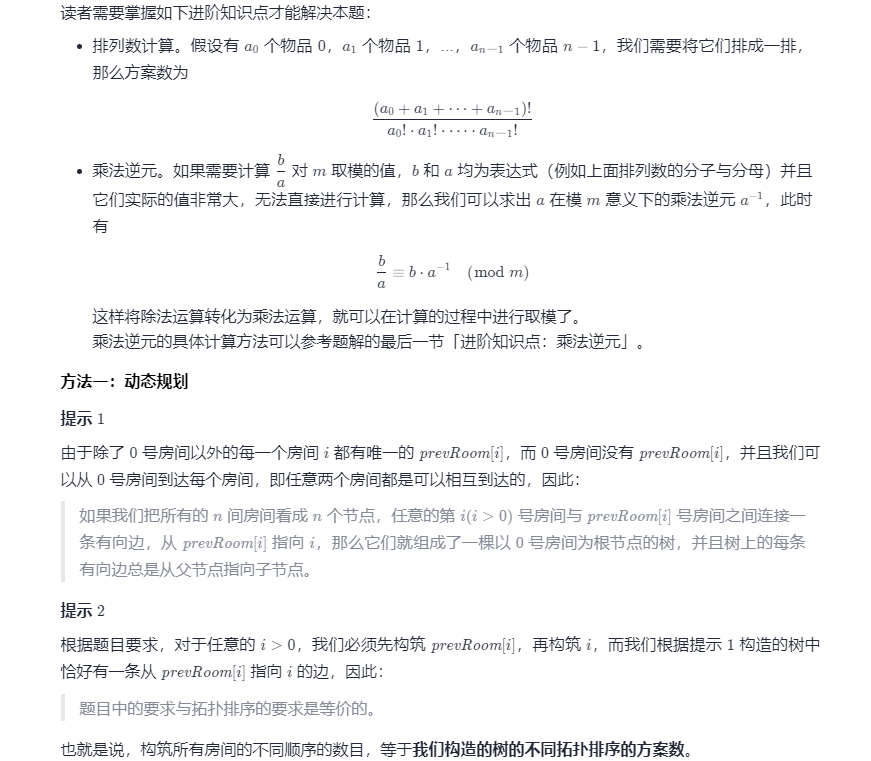
\includegraphics[width=.9\linewidth]{./pic/ant1.png}

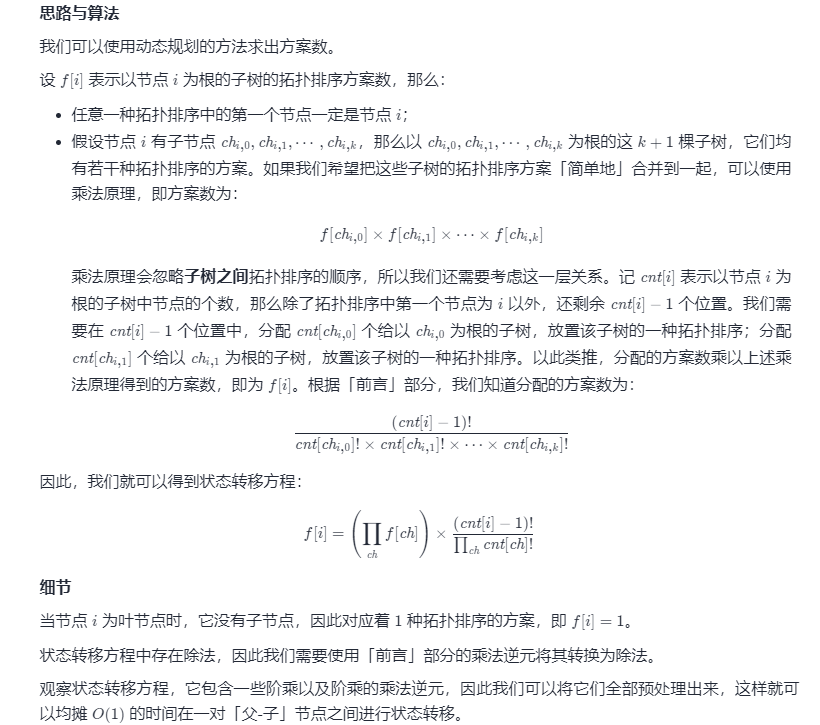
\includegraphics[width=.9\linewidth]{./pic/ant2.png}

\begin{minted}[frame=lines,fontsize=\scriptsize,linenos=false]{java}
// 快速计算x^y的乘方
public int quickMul(int x , int y) {
    long res = 1, cur = x;
    while (y > 0) {
        if ((y & 1) == 1)
            res = res * cur % mod;
        cur = cur * cur % mod;
        y >>= 1;
    }
    return (int)res;
}
// 深度优先搜索,返回以当前节点为根的子树节点个数 及 内部排列数
public int [] dfs (int idx) {
    if (!map.containsKey(idx)) return new int [] {1, 1}; // 子节点,节点个数及内部排列数均为1
    int cnt = 1, res = 1;       //  子树的节点个数、内部排列数
    for (Integer node : map.get(idx)) {
      int [] cur = dfs(node); // 递归得到子节点对应树的节点个数和排列数
        cnt += cur[0];
        res = (int)((long)res * cur[1] % mod * inv[cur[0]] % mod);
    }
    res = (int)((long)res * fac[cnt-1] % mod);
    return new int [] {cnt, res};
}
int mod = (int)1e9 + 7;
Map<Integer, List<Integer>> map = new HashMap<>();
int [] fac, inv;
public int waysToBuildRooms(int[] prevRoom) {
    int n = prevRoom.length;
    // 求阶乘数列及对应逆元
    this.fac = new int [n]; // fac[i]=i!
    this.inv = new int [n]; // inv[i]=i!^(-1)
    fac[0] = inv[0] = 1;
    for (int i = 1; i < n; i++) {
        fac[i] = (int)((long)fac[i-1] * i % mod);
        inv[i] = quickMul(fac[i], mod - 2); // 费马小定理: (fac[i]^(-1))%mod = (fac[i]^(mod-2))%mod
    }
    // 记录各个节点与子节点之间的边
    for (int i = 1; i < n; i++) 
        map.computeIfAbsent(prevRoom[i], k->new ArrayList<>()).add(i);
    // 动态规划得到总体顺序数量x
    return dfs(0)[1];      
}
\end{minted}

\section{1987. Number of Unique Good Subsequences - Hard}
\label{sec-1-9}
You are given a binary string binary. A subsequence of binary is considered good if it is not empty and has no leading zeros (with the exception of "0").

Find the number of unique good subsequences of binary.

For example, if binary = "001", then all the good subsequences are ["0", "0", "1"], so the unique good subsequences are "0" and "1". Note that subsequences "00", "01", and "001" are not good because they have leading zeros.
Return the number of unique good subsequences of binary. Since the answer may be very large, return it modulo 109 + 7.

A subsequence is a sequence that can be derived from another sequence by deleting some or no elements without changing the order of the remaining elements.
\begin{minted}[frame=lines,fontsize=\scriptsize,linenos=false]{java}
public int numberOfUniqueGoodSubsequences(String binary) {
    int mod = (int)1e9 + 7;
    int n = binary.length(), preZoo = 0, preOne = 0, m = 1;
    long [] dp = new long [n+1];
    String s = "#" + binary;
    while (m <= n && s.charAt(m) == '0') m++;
    if (m == n+1) return 1;
    dp[m] = 1;
    preOne = m;
    preZoo = m-1;
    for (int i = m+1; i <= n; i++) {
        char c = s.charAt(i);
        int j = (c == '0' ? preZoo : preOne);
        dp[i] = (2 * dp[i-1] % mod - (j >= 1 ? dp[j-1] : 0) + mod) % mod;
        if (c == '0') preZoo = i;
        else preOne = i;
    }
    return (int)dp[n] + (s.indexOf("0") != -1 ?  1 : 0);
}
\end{minted}
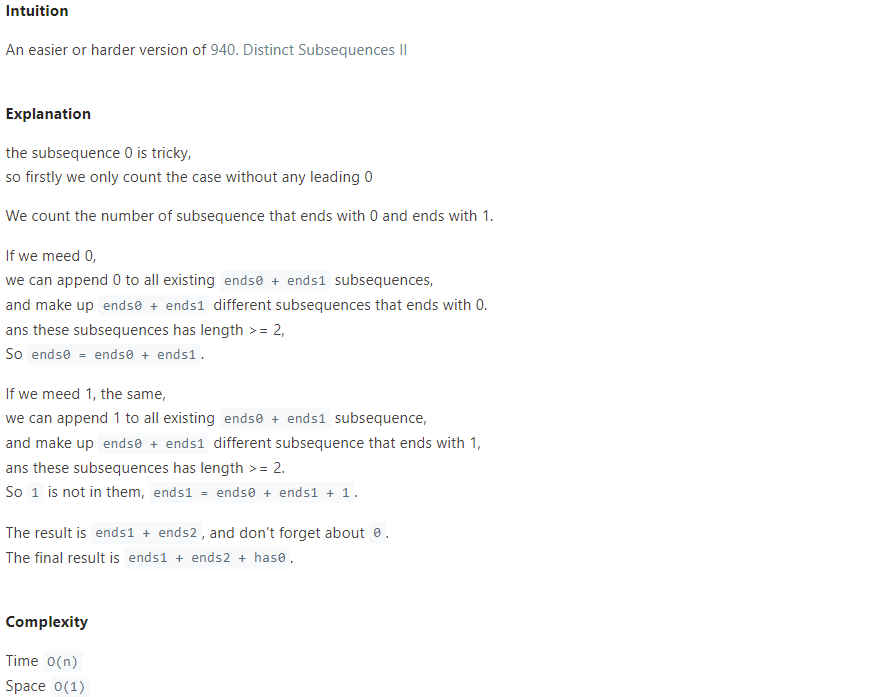
\includegraphics[width=.9\linewidth]{./pic/distinctSubsequence.png}
\begin{minted}[frame=lines,fontsize=\scriptsize,linenos=false]{java}
public int numberOfUniqueGoodSubsequences(String binary) {
    int mod = (int)1e9 + 7;
    int endZoo = 0, endOne = 0, hasZoo = 0;
    for (int i = 0; i < binary.length(); i++) 
        if (binary.charAt(i) == '1')
            endOne = (endOne + endZoo + 1) % mod;
        else {
            endZoo = (endZoo + endOne) % mod;
            hasZoo = 1;
        }
    return (endOne + endZoo + hasZoo) % mod;
}
\end{minted}
\begin{itemize}
\item 还有一个没有看懂的
\begin{itemize}
\item \url{https://leetcode-cn.com/problems/number-of-unique-good-subsequences/solution/ju-yi-fan-san-by-avenger-h-34xa/}
\item \url{https://leetcode-cn.com/problems/distinct-subsequences-ii/solution/dong-tai-gui-hua-cong-fen-xi-dao-shi-xian-by-my10y/}
\end{itemize}
\end{itemize}
\begin{minted}[frame=lines,fontsize=\scriptsize,linenos=false]{python}
def numberOfUniqueGoodSubsequences(self, binary: str) -> int:
        M = 10**9+7
        dp = [0]*10
        b = str(int(binary))
        l = len(binary) - len(b)
        if l > 0:
            dp[0] = 1
        for c in b:
            if dp[0] >= 1:
                dp[int(c)] = (sum(dp)) % M
            else:
                dp[int(c)] = ( 1+ sum(dp)) % M
        return sum(dp)%M
\end{minted}
\section{730. Count Different Palindromic Subsequences - Hard}
\label{sec-1-10}
Given a string s, return the number of different non-empty palindromic subsequences in s. Since the answer may be very large, return it modulo 109 + 7.

A subsequence of a string is obtained by deleting zero or more characters from the string.

A sequence is palindromic if it is equal to the sequence reversed.

Two sequences a1, a2, \ldots{} and b1, b2, \ldots{} are different if there is some i for which ai != bi.

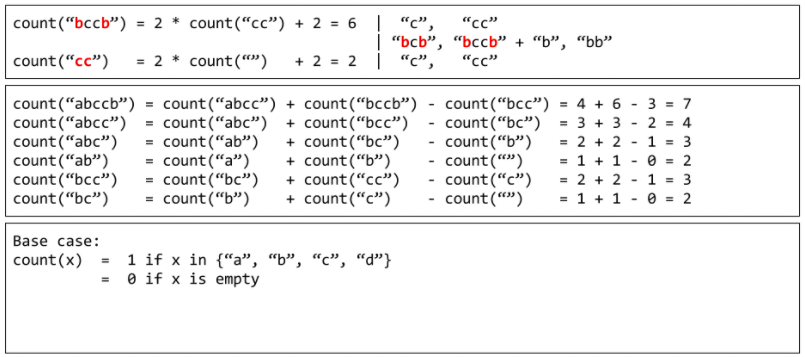
\includegraphics[width=.9\linewidth]{./pic/palindromSubSeq.png}

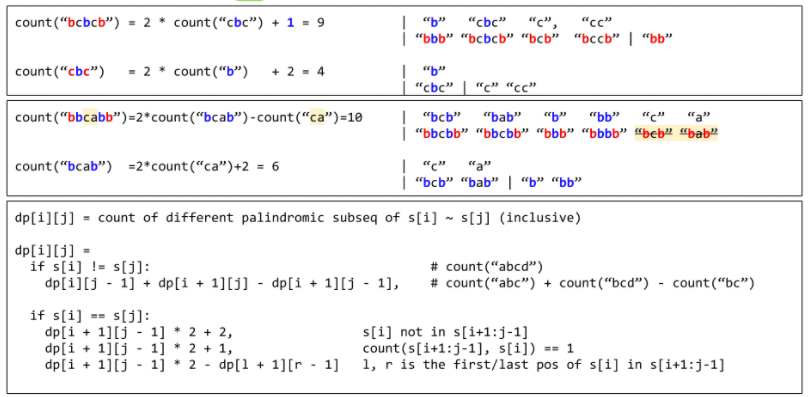
\includegraphics[width=.9\linewidth]{./pic/palindromSubSeq2.png}

\begin{minted}[frame=lines,fontsize=\scriptsize,linenos=false]{java}
private int dfs(char[] s, int i, int j) {
    if (i > j) return 0;
    if (i == j) return 1;
    if (dp[i][j] > 0) return dp[i][j];
    long ans = 0;
    if (s[i] == s[j]) {
        ans += dfs(s, i + 1, j - 1) * 2;
        int l = i + 1;
        int r = j - 1;
        while (l <= r && s[l] != s[i]) ++l;
        while (l <= r && s[r] != s[i]) --r;
        if (l > r) ans += 2;
        else if (l == r) ans += 1;
        else ans -= dfs(s, l + 1, r - 1);
    } else 
        ans = dfs(s, i, j - 1) + dfs(s, i + 1, j) - dfs(s, i + 1, j - 1);
    return dp[i][j] = (int)((ans + mod) % mod);
}
private static final int mod = (int)1e9 + 7;
private int [][] dp;
public int countPalindromicSubsequences(String S) {
    int n = S.length();
    dp = new int[n][n];
    return dfs(S.toCharArray(), 0, n - 1);
}
\end{minted}
\begin{itemize}
\item dp
\end{itemize}
\begin{minted}[frame=lines,fontsize=\scriptsize,linenos=false]{java}
public int countPalindromicSubsequences(String s) {
    int n = s.length();
    int mod = (int)1e9 + 7;
    char [] arr = s.toCharArray();
    long [][] dp = new long [n][n];
    for (int i = 0; i < n; i++) 
        dp[i][i] = 1;
    for (int len = 1; len <= n; len++) {
        for (int i = 0; i+len < n; i++) {
            int j = i + len;
            if (arr[i] == arr[j]) {
                dp[i][j] = dp[i+1][j-1] * 2;
                int l = i+1;
                int r = j-1;
                while (l <= r && arr[l] != arr[i]) ++l;
                while (l <= r && arr[r] != arr[i]) --r;
                if (l == r) dp[i][j] += 1;
                else if (l > r) dp[i][j] += 2;
                else dp[i][j] -= dp[l+1][r-1];
            } else dp[i][j] = dp[i][j-1] + dp[i+1][j] - dp[i+1][j-1];
            dp[i][j] = (dp[i][j] + mod) % mod;
        }
    }
    return (int)dp[0][n-1];
}
\end{minted}

\section{1125. Smallest Sufficient Team - Hard 这个题要多写几遍}
\label{sec-1-11}
In a project, you have a list of required skills req$_{\text{skills}}$, and a list of people. The ith person people[i] contains a list of skills that the person has.

Consider a sufficient team: a set of people such that for every required skill in req$_{\text{skills}}$, there is at least one person in the team who has that skill. We can represent these teams by the index of each person.

For example, team = [0, 1, 3] represents the people with skills people\footnotemark[2]{}, people\footnote{DEFINITION NOT FOUND.}, and people\footnotemark[1]{}.
Return any sufficient team of the smallest possible size, represented by the index of each person. You may return the answer in any order.

It is guaranteed an answer exists.
\begin{minted}[frame=lines,fontsize=\scriptsize,linenos=false]{java}
// 强行剪枝: 收集到的size >= 目前的结果,直接return;
// 这题的思路就是先把skill 和set of people建立好,
// 然后去用skill set做backtracking收集,如果temp team的size大于结果,直接return,否则update结果,
// 这里有个小tricky的地方,就是如果people是新人,加入之后dfs,backtracking的时候,要判断如果是新人,则remove,否则不remove;
private void dfs(String[] req_skills, HashSet<Integer> team, int idx) {
    if (team.size() >= minTeamSize) return; // 强行剪枝: 收集到的size >= 目前的结果,直接return;
    if (idx == req_skills.length) {
        minTeamSize = team.size();
        resTeam = new HashSet<Integer>(team);
        return;
    }
    boolean isNewPerson = false;
    for (int people : map.get(req_skills[idx])) {
        isNewPerson = team.add(people);
        dfs(req_skills, team, idx + 1);
        if (isNewPerson)
            team.remove(people);
    }
}
HashMap<String, Set<Integer>> map;
Set<Integer> resTeam; 
int minTeamSize;
public int[] smallestSufficientTeam(String[] req_skills, List<List<String>> people) {
    minTeamSize = people.size();
    this.map = new HashMap<>(); 
    for (int i = 0; i < minTeamSize; i++) 
        for (String skill: people.get(i)) 
            map.computeIfAbsent(skill, k -> new HashSet<Integer>()).add(i);
    this.resTeam = new HashSet<Integer>();
    dfs(req_skills, new HashSet<Integer>(), 0);
    int [] res = new int[resTeam.size()];     
    int idx = 0;
    for (int person : resTeam) 
        res[idx++] = person;
    return res;
}
\end{minted}
\begin{itemize}
\item Java soution using Bit DP 10ms
\end{itemize}
\begin{minted}[frame=lines,fontsize=\scriptsize,linenos=false]{java}
public int[] smallestSufficientTeam(String[] req_skills, List<List<String>> people) {
    int n = req_skills.length, range = 1 << n, cur, idx;
    Map<String, Integer> idxMap = new HashMap<>();
    for (int i = 0; i < n; i++) 
        idxMap.put(req_skills[i], i);
    long [] dp = new long [range]; // 每个bit位实际存了构成答案最小组的各成员的下标, 60个人, long
    int [] cnt = new int [range];
    Arrays.fill(cnt, Integer.MAX_VALUE);
    cnt[0] = 0;
    for (int i = 0; i < people.size(); i++) {
        List<String> l = people.get(i);
        cur = 0;
        for (String skill : l) 
            if (idxMap.containsKey(skill))
                cur |= 1 << idxMap.get(skill);
        for (int j = range-1; j > 0; j--) {
            idx = (j & cur) ^ j; // 由其它人所构成的拥有j的这些种技能的子集/ j的这些种技能可以由j一个人来替换(其它可能需要很多人才能最终拥有这些技能)
            if (cnt[idx] != Integer.MAX_VALUE && cnt[j] > cnt[idx] + 1) {
                cnt[j] = cnt[idx] + 1;
                dp[j] = dp[idx] | (1L << i); // at most 60 people
            }
        }
    }
    int [] res = new int[cnt[range-1]];
    long preRes = dp[range-1]; // 5 people: 11111, 1111, 111, 11, 1
    int valIdx = 0;
    long val = 0;
    idx = 0;
    while (preRes != 0) {
        val = preRes & 1;
        if (val == 1) res[idx++] = valIdx;
        preRes >>= 1;
        valIdx++;
    }
    return res;
}
\end{minted}
\begin{itemize}
\item DFS + Memorizaion (A real O(2$^{\text{skill}}$ * people) Solution) Java 8ms
\begin{itemize}
\item \url{https://leetcode.com/problems/smallest-sufficient-team/discuss/1011135/DFS-\%2B-Memorizaion}-(A-real-O(2skill-*-people)-Solution)-Java-8ms
\end{itemize}
\end{itemize}
\begin{minted}[frame=lines,fontsize=\scriptsize,linenos=false]{java}
List<Integer> minComb;
int[] peopleSkillMasks;
Integer[] memo;  // 这个方法确实快一点儿
int[] nextPerson;
int n;
public int[] smallestSufficientTeam(String[] req_skills, List<List<String>> people) {
    // 1. some preprocess to get bitmask for people skills
    this.n = req_skills.length;
    Map<String, Integer> skillToIdx = new HashMap<>();
    for (int i = 0; i < n; i++) 
        skillToIdx.put(req_skills[i], i);
    this.peopleSkillMasks = new int[people.size()];
    for (int i = 0; i < peopleSkillMasks.length; i++) {
        int skillMask = 0;
        for (String skill : people.get(i)) 
            skillMask |= (1 << skillToIdx.get(skill));
        peopleSkillMasks[i] = skillMask;
    }
    // 2. dfs
    memo = new Integer[1 << n];
    nextPerson = new int[1 << n];
    dfs(0, 0);
    // 3. reconstruct the path
    int curSkillSet = 0;
    List<Integer> res = new ArrayList<>();
    while(curSkillSet != (1 << n) - 1) {
        res.add(nextPerson[curSkillSet]);
        curSkillSet |= peopleSkillMasks[nextPerson[curSkillSet]];
    }
    return res.stream().mapToInt(i->i).toArray();
}
// a very simple dfs with memo to compute all combinations of people. 
// Use memorization to optimize the time complexity to O(2^skill * people) 2^skill for 2^skill node in the tree, people because each node has people computation
private int dfs(int curSkillSet, int startIdx) {
    if (curSkillSet == (1 << n) - 1) return 0;
    if (memo[curSkillSet] == null) {
        int res = Integer.MAX_VALUE / 2;
        int nextPersonIdx = -1;
        for (int i = startIdx; i < peopleSkillMasks.length; i++) {
            int withNewSkill = peopleSkillMasks[i] | curSkillSet; 
            if (withNewSkill != curSkillSet) {
                int numPeople = dfs(withNewSkill, i+1) + 1;
                if (res > numPeople) {
                    res = numPeople;
                    nextPersonIdx = i;
                }
            }
        }
        memo[curSkillSet] = res;
        nextPerson[curSkillSet] = nextPersonIdx; 
    }
    return memo[curSkillSet];
}
\end{minted}
\begin{itemize}
\item Recursion + Memoization + bit mask , with Simple JAVA solution
\begin{itemize}
\item \url{https://leetcode.com/problems/smallest-sufficient-team/discuss/1487180/Recursion-\%2B-Memoization-\%2B-bit-mask-with-Simple-JAVA-solution}
\end{itemize}
\end{itemize}
上面的这些方法相对较偏,就暂时顾不上了

\section{1575. Count All Possible Routes - Hard}
\label{sec-1-12}
You are given an array of distinct positive integers locations where locations[i] represents the position of city i. You are also given integers start, finish and fuel representing the starting city, ending city, and the initial amount of fuel you have, respectively.

At each step, if you are at city i, you can pick any city j such that j != i and 0 <= j < locations.length and move to city j. Moving from city i to city j reduces the amount of fuel you have by |locations[i] - locations[j]|. Please notice that |x| denotes the absolute value of x.

Notice that fuel cannot become negative at any point in time, and that you are allowed to visit any city more than once (including start and finish).

Return the count of all possible routes from start to finish.

Since the answer may be too large, return it modulo 10$^{\text{9}}$ + 7.
\begin{minted}[frame=lines,fontsize=\scriptsize,linenos=false]{java}
// 自顶向下 (记忆化搜索)
// 每个dfs搜索当前状态为城市i,油量f到达终点的方案数。这样决策的时候就很直观:当前这个状态的方案数,由可去的城市的,且油量为剩余油量的到达终点方案数加起来。
// 初始化:每个状态都初始化为-1。
// 当走到终点时,这个状态的可走到终点的方案数+1。
private int dfs(int [] arr, int end, int idx, int fu) {
    if (dp[idx][fu] != -1) return dp[idx][fu];
    dp[idx][fu] = 0;
    if (idx == end) {
        dp[idx][fu] += 1;
        dp[idx][fu] %= mod;
    }
    for (int i = 0; i < n; i++) {
        if (i == idx || Math.abs(arr[i] - arr[idx]) > fu) continue;
        dp[idx][fu] = (dp[idx][fu] + dfs(arr, end, i, fu-Math.abs(arr[i]-arr[idx]))) % mod;
    }
    return dp[idx][fu];
}
int mod = (int)1e9 + 7;
int [][] dp;
int n;
public int countRoutes(int[] locations, int start, int finish, int fuel) {
    n = locations.length;
    if (fuel < Math.abs(locations[start] - locations[finish])) return 0;
    dp = new int[n][fuel+1];
    for (int i = 0; i < n; i++) 
        Arrays.fill(dp[i], -1);
    dfs(locations, finish, start, fuel);
    return dp[start][fuel];
}
// 自底向上
// 为什么想到动态规划:最优子结构:到达终点的方案数肯定由到达其他点的,不同油量的方案数求和。
//     如何定义状态:城市肯定在状态里,因为其他城市有不同的剩余油量的状态,且油量为0无法到达,也成为限制之一。所以油量也必须在状态里:
//     d p ( i , f ) dp(i, f)dp(i,f)表示到达第 i ii个城市,剩余油量为f ff 的方案数。
//     状态转移:第i ii个城市,可以由除本身外的城市转移过来,只要剩余的油量不小于所用的油量就够了,最后答案是求总共的个数,所以只要方案数相加就行:
//     dp(i,f−dist)=dp(i,f−dist)+dp(k,f)(f−dist>=0)
//     枚举顺序:每个城市肯定都要枚举一遍,因为还需要从另一个城市转移过来,所以除本身外的城市肯定还要再枚举一遍。
//     关键是油量的枚举,因为油量肯定是慢慢减少的,可以想到是逆序枚举,而且油量要放在最外层枚举。因为如果先枚举城市i ii,再枚举城市j jj,再枚举油量的话,只是不断更新了i ii城市方案数,而j jj城市不同油量的方案数根本没变化。
// dp:最优子结构 到达终点的方案数肯定由到达其他点的,不同油量的方案数求和
// 搜索:反过来 在第 i 个城市到达 fin 的方案数,也可以由其他的点到达 fin 的方案数转移过来, 但是油量有限制,所以油量肯定在状态里
// 所以城市 和 剩余油量肯定在状态里
// dp(i, j) 表示到达第 i 个城市,剩余油量为 j 的方案数
// dp(i, j) = dp(i, j) + dp(k, j - dist)
public int countRoutes(int[] locations, int start, int finish, int fuel) {
    int n = locations.length;
    if (fuel < Math.abs(locations[start] - locations[finish])) return 0;
    int [][] dp = new int[n][fuel+1];
    dp[start][fuel] = 1; // 初始点且燃料满的点方案数为1
    int leftFu = 0, mod = (int)1e9 + 7;
    for (int j = fuel; j >= 0; j--) { // fuel leftover
        for (int i = 0; i < n; i++) { // cur city
            for (int k = 0; k < n; k++) { // next city
                if (i == k) continue;
                leftFu = j - Math.abs(locations[i] - locations[k]);
                if (leftFu < 0) continue;
                dp[i][leftFu] = (dp[i][leftFu] + dp[k][j]) % mod; // 这里好别扭呀: 想呀想呀 
            }
        }
    }
    int ans = 0;
    for (int i = 0; i <= fuel; i++) 
        ans = (ans + dp[finish][i]) % mod;
    return ans;
}
\end{minted}

\section{1012. Numbers With Repeated Digits - Hard}
\label{sec-1-13}
Given an integer n, return the number of positive integers in the range [1, n] that have at least one repeated digit.

题意:统计1-N中,满足每个位置都不同的数有几个。

思路:数位DP。通过一个1<<10的mask表示当前这个数,1-9哪些数被用了。

比赛的时候,一直想通过一个dfs直接找到不重复的数,一直不对。

赛后发现,别人都是通过一个dfs找重复的数,然后总个数减去。

\begin{minted}[frame=lines,fontsize=\scriptsize,linenos=false]{java}
private int dfs(int len, int limit, int mask) { // 不重复数的个数
    if (len == 0) return 1;
    if (limit == 0 && dp[len][mask][limit] > 0) return dp[len][mask][limit]; // 记忆化部分
    int maxn = limit > 0 ? bit[len] : 9; // 求出最高可以枚举到哪个数字
    int ans = 0;
    for (int i = 0; i <= maxn; i++)  // 当前位
        if ((mask&(1 << i)) == 0)
            if (mask == 0 && i == 0)
                ans += dfs(len - 1, (limit > 0 && i == maxn ? 1 : 0), mask); // 有前导0,所以0不能统计,不更新mask
            else ans += dfs(len - 1, (limit > 0 && i == maxn ? 1 : 0), mask | (1 << i)); // 更新mask
    if (limit == 0) dp[len][mask][limit] = ans; // 如果没有限制,代表搜满了,可以记忆化,否则就不能
    return ans;
}
int [][][] dp;
int [] bit;
public int numDupDigitsAtMostN(int N) {
    int sum = N + 1;
    bit = new int [19];
    dp = new int [19][1 << 10][2];
    int idx = 0;
    while (N > 0) {
        bit[++idx] = N % 10;
        N /= 10;
    }
    return sum - dfs(idx, 1, 0);
}
\end{minted}
\begin{itemize}
\item 这道题给了一个正整数N,让返回所有不大于N且至少有一个重复数字的正整数的个数,题目中给的例子也可以很好的帮助我们理解。要求的是正整数的位数上至少要有一个重复数字,当然最简单暴力的方法就是从1遍历到N,然后对于每个数字判断是否有重复数字,看了一眼题目难度 Hard,想都不用想,肯定是超时的。这道题需要更高效的解法,首先来想,若是直接求至少有一个重复数字的正整数,由于并不知道有多少个重复数字,可能1个,2个,甚至全是重复数字,这样很难找到规律。有时候直接求一个问题不好求,可以考虑求其相反的情况,至少有一个重复数字反过来就是一个重复数字都没有,所以这里可以求不大于N且一个重复数字都没有的正整数的个数,然后用N减去这个数字即为所求。好,接下来看怎么求,对于任意一个N,比如 7918,是个四位数,而所有的三位数,两位数,一位数,都一定比其小,所以可以直接求出没有重复数字的三位数,两位数,和一位数。比如三位数,由于百位上不能有0,则只有9种情况,十位上可以有0,则有9种情况,个位上则有8种情况,所以就是 9*9*8。可以归纳出没有重复数字的n位数的个数,最高位去除0还有9种,剩余的 n-1 位则依次是 9,8,7\ldots{} 则后面的 n-1 位其实是个全排列,从9个数中取出 n-1 个数字的全排列,初中就学过的。这里写一个全排列的子函数,求从m个数字中取n个数字的全排列,方便后面计算。算完这些后,还要来算符合题意的四位数,由于第一位是7,若千位上是小于7的数字(共有6种,千位上不能是0),则后面的百位,十位,个位又都可以全排列了,从9个数字中取3个数字的全排列,再乘以千位上小于7的6种情况。若当千位固定为7,则百位上可以放小于9的数字(共有8种,百位不能放7,但可以放0),则后面的十位和个位都可以全排列了,从8个数字种取出2个数字的全排列,再乘以百位上小于9的8种情况。需要注意的是,遍历给定数字的各个位时,有可能出现重复数字,一旦出现了之后,则该 prefix 就不能再用了,因为已经不合题意了。所以要用一个 HashSet 来记录访问过的数字,一旦遇到重复数字后就直接 break 掉。最后还有一个小 trick 需要注意,由于N本身也需要计算进去,所以再计算的时候,使用 N+1 进行计算的话,就可以把N这种情况算进去了
\end{itemize}
\begin{minted}[frame=lines,fontsize=\scriptsize,linenos=false]{java}
private int A(int m, int n) {
    return n == 0 ? 1 : A(m, n-1) * (m-n+1);
}
public int numDupDigitsAtMostN(int n) {
    List<Integer> digits = new ArrayList<>();
    Set<Integer> vis = new HashSet<>();
    for (int i = n+1; i > 0; i /= 10) 
        digits.add(0, i % 10);
    int res = 0, m = digits.size();
    for (int i = 1; i < m; i++) res += 9 * A(9,  i-1);
    for (int i = 0; i < m; i++) {
        for (int j = i > 0 ? 0 : 1; j < digits.get(i); ++j) {
            if (vis.contains(j)) continue;
            res += A(9-i, m-i-1);
        }
        if (vis.contains(digits.get(i))) break;
        vis.add(digits.get(i));
    }
    return n - res;
}
\end{minted}

\section{514. Freedom Trail - Hard}
\label{sec-1-14}
In the video game Fallout 4, the quest "Road to Freedom" requires players to reach a metal dial called the "Freedom Trail Ring" and use the dial to spell a specific keyword to open the door.

Given a string ring that represents the code engraved on the outer ring and another string key that represents the keyword that needs to be spelled, return the minimum number of steps to spell all the characters in the keyword.

Initially, the first character of the ring is aligned at the "12:00" direction. You should spell all the characters in key one by one by rotating ring clockwise or anticlockwise to make each character of the string key aligned at the "12:00" direction and then by pressing the center button.

At the stage of rotating the ring to spell the key character key[i]:

You can rotate the ring clockwise or anticlockwise by one place, which counts as one step. The final purpose of the rotation is to align one of ring's characters at the "12:00" direction, where this character must equal key[i].
If the character key[i] has been aligned at the "12:00" direction, press the center button to spell, which also counts as one step. After the pressing, you could begin to spell the next character in the key (next stage). Otherwise, you have finished all the spelling.
\subsection{解题思路分析: 这个图把钥匙中每个字母的出现位置记住了,以后拿去用不搜 dfs + 记忆数组}
\label{sec-1-14-1}
\begin{itemize}
\item 记录下所有字母对应的位置,这样在找字母相对位置的时候就不需要循环搜索了
\item 采用递归的方法,找出当前字母对应的位置最小的步数:只需要把当前字母对应的所有位置找出来,然后计算最小值即可
\item 下一个位置再次迭代计算即可
\end{itemize}
\begin{minted}[frame=lines,fontsize=\scriptsize,linenos=false]{java}
public int minLen(int len, int i, int j) {
    int min = Math.min(i, j);
    int max = Math.max(i, j);
    return Math.min(Math.abs(i - j), Math.abs(len + min - max));
}
public int helper(String ring, int i, String key, int j) {
    if (j >= n) return 0;
    if (dp[i][j] > 0) return dp[i][j];
    List<Integer> nextPos = map.get(key.charAt(j));
    int min = Integer.MAX_VALUE;
    for (int k = 0; k < nextPos.size(); k++) 
        min = Math.min(min, helper(ring, nextPos.get(k), key, j+1) + minLen(m, nextPos.get(k), i) + 1);
    dp[i][j] = min;
    return dp[i][j];
}
Map<Character, List<Integer>> map = new HashMap<>(); // 这个图把钥匙中每个字母的出现位置记住了,以后拿去用不搜
int[][] dp;
int m, n;
public int findRotateSteps(String ring, String key) {
    m = ring.length();
    n = key.length();
    dp = new int[m][n];
    for (int i = 0; i < m; i++) {
        if (key.indexOf(ring.charAt(i)) == -1) continue;
        char c = ring.charAt(i);
        List<Integer> li = map.get(c);
        if (li == null) {
            li = new ArrayList<>();
            map.put(c, li);
        }
        li.add(i);
    }
    return helper(ring, 0, key, 0);
}
\end{minted}
\subsection{解题思路分析 动态规划}
\label{sec-1-14-2}
\begin{itemize}
\item 博主最先尝试的用贪婪算法来做,就是每一步都选最短的转法,但是OJ中总有些test case会引诱贪婪算法得出错误的结果,因为全局最优解不一定都是局部最优解,而贪婪算法一直都是在累加局部最优解,这也是为啥DP解法这么叼的原因。贪婪算法好想好实现,但是不一定能得到正确的结果。DP解法难想不好写,但往往才是正确的解法,这也算一个trade off吧。
\item 此题需要使用一个二维数组dp,其中dp[i][j]表示转动从i位置开始的key串所需要的最少步数(这里不包括spell的步数,因为spell可以在最后统一加上),此时表盘的12点位置是ring中的第j个字符。不得不佩服这样的设计的确很巧妙,我们可以从key的末尾往前推,这样dp\footnotemark[2]{}\textsuperscript{,}\,\footnotemark[2]{}就是我们所需要的结果,因为此时是从key的开头开始转动,而且表盘此时的12点位置也是ring的第一个字符。现在我们来看如何找出递推公式,对于dp[i][j],我们知道此时要将key[i]转动到12点的位置,而此时表盘的12点位置是ring[j],我们有两种旋转的方式,顺时针和逆时针,我们的目标肯定是要求最小的转动步数,而顺时针和逆时针的转动次数之和刚好为ring的长度n,这样我们求出来一个方向的次数,就可以迅速得到反方向的转动次数。为了将此时表盘上12点位置上的ring[j]转动到key[i],我们要将表盘转动一整圈,当转到key[i]的位置时,我们计算出转动步数diff,然后计算出反向转动步数,并取二者较小值为整个转动步数step,此时我们更新dp[i][j],更新对比值为step + dp[i+1][k],这个也不难理解,因为key的前一个字符key[i+1]的转动情况suppose已经计算好了,那么dp[i+1][k]就是当时表盘12点位置上ring[k]的情况的最短步数,step就是从ring[k]转到ring[j]的步数,也就是key[i]转到ring[j]的步数,用语言来描述就是,从key的i位置开始转动并且此时表盘12点位置为ring[j]的最小步数(dp[i][j])就等价于将ring[k]转动到12点位置的步数(step)加上从key的i+1位置开始转动并且ring[k]已经在表盘12点位置上的最小步数(dp[i+1][k])之和。
\item 突然发现这不就是之前那道Reverse Pairs中解法一中归纳的顺序重现关系的思路吗,都做了总结,可换个马甲就又不认识了,泪目中。。。
\end{itemize}
\begin{minted}[frame=lines,fontsize=\scriptsize,linenos=false]{java}
public int findRotateSteps(String ring, String key) {
    int m = key.length(); 
    int n = ring.length();
    int [][] dp = new int[m+1][n];
    int diff = 0, step = 0;
    for (int i = m-1; i >= 0; i--) {
        for (int j = 0; j < n; j++) {
            dp[i][j] = Integer.MAX_VALUE;
            for (int k = 0; k < n; k++) {
                if (ring.charAt(k) == key.charAt(i)) {
                    diff = Math.abs(j - k);
                    step = Math.min(diff, n-diff);
                    dp[i][j] = Math.min(dp[i][j], step + dp[i+1][k]);
                }
            }
        }
    }
    return dp[0][0] + m;
}
\end{minted}

\subsection{解题思路分析: dfs + 记忆数组}
\label{sec-1-14-3}
\begin{itemize}
\item 过程就是需要一步一步求key里面的每个字符。 如果当前位置已经是对应到这个字符,那么直接按按钮就可以
\item 如果当前位置不是,那么有两种旋转方式,顺时针或者逆时针, 然后找到第一个字符就是在同一个方向上的最短距离,
\item 因为在同一个方向上,即使后面有重复的字符,无论后面的字符在那里,遇到第一个符合条件的字符就按按钮一定是最优解。
\item 但是在不同方向上就不一定了,有可能一个方向上当前字符距离更短,但是有可能后面的字符距离会更远,
\begin{itemize}
\item 比如ring=ABCDEFGBF , key=BG, 如果看第一个字符, 那应该是顺时针,只需要转一格就到,逆时针需要转两格,
\item 但是顺时针第一步快了以后, 后面到G会需要更长的步骤。 而逆时针会比较快。
\end{itemize}
\item 所以,基本的逻辑是每一步不能决定当前哪个方向是否是最优解, 只有不断递归,把每步的两个方向全部尝试完到key结束才可以
\item 当然, 如果不做任何处理,这样做是要超时的(我开始就写了这样一个版本), 一个直观的做法,就是在递归的基础上
\begin{itemize}
\item 加一个记忆表, 针对ring的位置index和key的kindex做记录, 如果已经存在一个解了就可以直接返回结果
\end{itemize}
\item 这个递归+memorization的解法,那一定存在一个bottom up的动态规划解法, 这个后面再学习
\end{itemize}
\begin{minted}[frame=lines,fontsize=\scriptsize,linenos=false]{java}
private int helper(String s, String t, int i, int j) { // s: ring, t: key, i: idxRing, j: idxKey
    Map<Integer, Integer> locMap = mem.get(i);
    if (locMap != null) 
        if (locMap.get(j) != null) return locMap.get(j);
    if (j == n) return 0;
    int step = 0, k = i;
    boolean foundK = false;
    for (; step <= m/2; ++step) {
        k = (i + step + m) % m;
        if (s.charAt(k) == t.charAt(j)) {
            foundK = true;
            break;
        }
    }
    int rstep = 0, x = i;
    boolean foundX = false;
    while (rstep <= m/2) {
        x = (i - rstep + m) % m;
        if (s.charAt(x) == t.charAt(j)) {
            foundX = true;
            break;
        }
        rstep++;
    }
    int min = Integer.MAX_VALUE;
    if (foundK) min = helper(s, t, k, j+1) + step + 1;
    if (foundX) min = Math.min(min, helper(s, t, x, j+1) + rstep + 1);
    if (locMap == null) {
        locMap = new HashMap<>();
        mem.put(i, locMap);
    }
    locMap.put(j, min);
    return min;
}
Map<Integer, Map<Integer, Integer>> mem = new HashMap<>();
int m, n;
public int findRotateSteps(String ring, String key) {
    m = ring.length();
    n = key.length();
    return helper(ring, key, 0, 0);
}
\end{minted}

\section{847. Shortest Path Visiting All Nodes}
\label{sec-1-15}
You have an undirected, connected graph of n nodes labeled from 0 to n - 1. You are given an array graph where graph[i] is a list of all the nodes connected with node i by an edge.
Return the length of the shortest path that visits every node. You may start and stop at any node, you may revisit nodes multiple times, and you may reuse edges.
\begin{minted}[frame=lines,fontsize=\scriptsize,linenos=false]{java}
public int shortestPathLength(int[][] graph) {
    int n = graph.length;
    int tar = 0, res = 0;
    HashSet<String> s = new HashSet<>();
    Queue<Pair<Integer, Integer>> q = new LinkedList<>();
    for (int i = 0; i < n; i++) {
        int mask = (1 << i);
        tar |= mask;
        s.add(Integer.toString(mask) + "-" + Integer.toString(i));
        q.add(new Pair<>(mask, i));
    }
    while (!q.isEmpty()) {
        for (int i = q.size(); i > 0; i--) {
            Pair cur = q.remove();
            if ((int)cur.getKey() == tar) return res;
            for (int next : graph[(int)cur.getValue()]) {
                int path = (int)cur.getKey() | (1 << next);
                String str = Integer.toString(path) + "-" + Integer.toString(next);
                if (s.contains(str)) continue;
                s.add(str);
                q.add(new Pair<>(path, next));
            }
        }
        ++res;
    }
    return -1;
}
\end{minted}

\section{1931. Painting a Grid With Three Different Colors}
\label{sec-1-16}
You are given two integers m and n. Consider an m x n grid where each cell is initially white. You can paint each cell red, green, or blue. All cells must be painted.
Return the number of ways to color the grid with no two adjacent cells having the same color. Since the answer can be very large, return it modulo 109 + 7.
\begin{itemize}
\item lightweighted轻巧点儿的解题方案: bitmask
\end{itemize}
\begin{minted}[frame=lines,fontsize=\scriptsize,linenos=false]{java}
// time O( (2^5) *2 * N)
// SPACE O(N)
//     For m = 5, there are at most 48 valid states for a single column so we can handle it column by column.
//     We encode the color arrangement by bit mask (3 bit for a position) and use dfs to generate the all valid states.
//         Then for each column, we iterator all the states and check if its still valid with the previous column.
public void helper(int m, int pos, HashMap<Integer, Long> dic, int pre, int cur) {
    if (pos == m) {
        dic.put(cur, 1L);
        return;
    }
    //不需要{1, 2, 4} {0, 1, 2} is ok 每个格(实际占用3个bit)
    for (int i = 0; i < 3; i++) {
        if (i == pre) continue; 
        helper(m, pos + 1, dic, i, (cur << 3) | (1 << i)); // 每处理一格,将当前状态左移3位?(实际每个格占用3个bit位)| 现在这个格的值?这个,我好昏呀
    }
}
static int mod = (int) 1e9 + 7;
public int colorTheGrid(int m, int n) {
    HashMap<Integer,Long> dic = new HashMap<>();
    helper(m, 0, dic, -1, 0);     // 这应该就是我想找的精巧不占多少空间的mask了,可是有点儿看不懂
    HashSet<Integer> set = new HashSet<>(dic.keySet());
    for (int i = 1; i < n; i++) { // 动态规划: 用两个图像滚动数组一样轮流记载得出答案
        HashMap<Integer, Long> tmp = new HashMap<>();
        for (int x: set) 
            for (int y : set) 
                if ((x & y) == 0) // 相邻涂色方案为有效方案
                    tmp.put(y, (tmp.getOrDefault(y, 0L) + dic.get(x)) % mod);
        dic = tmp;
    }
    long res = 0L;
    for (Long x : dic.values()) {
        res += x;
        res %= mod;
    }
    return (int) res;
}
\end{minted}
\begin{itemize}
\item 比较传统一点儿的解法,思路清晰
\end{itemize}
\begin{minted}[frame=lines,fontsize=\scriptsize,linenos=false]{java}
// 参考的答案里,这个最逻辑简单、通俗大众易懂,但稍显笨重,两个图,用一个链表来记忆一行的涂色方案,如果有更精巧一点儿的bitmask,是我想找的答案
// https://leetcode.com/problems/painting-a-grid-with-three-different-colors/discuss/1334366/Easy-Java-comments-28ms-O(n*P*P)-complexity-memory-O(P)-where-P-is-column-permutations-count 这个又稍嫌太偏了,考得极少,不易懂,容易出错,可是bitmask又只能set 1 or 0,BitSet()可以吗?
// 先预处理得到单行的所有有效涂色方案,
// 再进一步计算得到每种单行方案对应的有效邻行方案
// 在此基础上,结合动态规划方法,逐行求解各种涂色状态对应的方案总数,最后统计得到总方案数。
public int colorTheGrid(int m, int n) {
// 获得单行所有涂色方案
    Map<Integer, List<Integer>> line = new HashMap<>(); //  3^m ways of paying one row
    int range = (int)Math.pow(3, m); // 用0、1、2表示各个网格的颜色,key为方案对应的数值,value为方案对应的数组
    for (int i = 0; i < range; i++) {
        List<Integer> list = new ArrayList<>(); //  val val values (0, 1, 2) of every m cols into list
        int val = i;
        for (int j = 0; j < m; j++) {
            list.add(val % 3);
            val /= 3;
        }
        boolean valid = true; // 确认该数组中是否存在相邻位置颜色相同
        for (int j = 1; j < m; j++) 
            if (list.get(j-1) == list.get(j)) {
                valid = false;
                break;
            }
        if (valid) line.put(i, list); // 相邻网格颜色均不同,为有效方案,加入哈希表
    }
// 预处理得到每种单行方案对应的有效邻行方案
    Map<Integer, List<Integer>> adj = new HashMap<>();
    Iterator it = line.entrySet().iterator();
    while (it.hasNext()) {     //  3^m ways of paying one row
        Map.Entry entry = (Map.Entry)it.next();
        int va = (int)entry.getKey();
        List<Integer> lva = (List<Integer>)entry.getValue();
        adj.put(va, new ArrayList<Integer>());
        Iterator itb = line.entrySet().iterator();
        while (itb.hasNext()) { //  3^m ways of paying one row
            Map.Entry enb = (Map.Entry)itb.next(); 
            int vb = (int)enb.getKey();
            List<Integer> lvb = (List<Integer>)enb.getValue();
            boolean valid = true;
            for (int i = 0; i < m; i++) 
                if (lva.get(i) == lvb.get(i)) {
                    valid = false;
                    break;
                } // among 3^m ways of painting one row, how many is valid, and valid mask into adj.get(va);
            if (valid) adj.get(va).add(vb); 
        }
    }
// 动态规划,逐行求解方案数
    int mod = (int)(1e9+7);
    long [] dp = new long [range];  // 上一行各种涂色方案对应的总方法数
    for (int i = 0; i < range; i++) // 初始化
        dp[i] = line.containsKey(i) ? 1 : 0;
    for (int i = 1; i < n; i++) {   // 从第二行开始动态规划
        long [] cur = new long [range];  // 新一行各种涂色方案对应的总方法数
        for (int j = 0; j < range; j++) 
            if (adj.containsKey(j)) {    // 该方案有效
                for (int v : adj.get(j)) // 遍历有效的相邻方案
                    cur[j] = (cur[j] + dp[v]) % mod; // 总方法数累加
            }
        System.arraycopy(cur, 0, dp, 0, range);
    }
    long ans = 0;
    for (int i = 0; i < range; i++) 
        ans = (ans + dp[i]) % mod;
    return (int)ans;
}
\end{minted}

\section{313. Super Ugly Number}
\label{sec-1-17}
A super ugly number is a positive integer whose prime factors are in the array primes.
Given an integer n and an array of integers primes, return the nth super ugly number.
The nth super ugly number is guaranteed to fit in a 32-bit signed integer.
\begin{minted}[frame=lines,fontsize=\scriptsize,linenos=false]{java}
static class Node implements Comparable<Node> {
    private int index;
    private int val;
    private int prime;
    public Node(int index, int val, int prime) {
        this.index = index;
        this.val = val;
        this.prime = prime;
    }
    public int compareTo(Node other) {
        return this.val - other.val;
    }
}
public int nthSuperUglyNumber(int n, int[] primes) {
    final int [] arr = new int[n];
    arr[0] = 1;              // 1 is the first ugly number
    final Queue<Node> q = new PriorityQueue<>();
    for (int i = 0; i < primes.length; ++i) 
        q.add(new Node(0, primes[i], primes[i]));
    for (int i = 1; i < n; ++i) {
        Node node = q.peek(); // get the min element and add to arr
        arr[i] = node.val;
        do {             // update top elements
            node = q.poll();
            node.val = arr[++node.index] * node.prime;
            q.add(node); // push it back
        } while (!q.isEmpty() && q.peek().val == arr[i]); // prevent duplicate
    }
    return arr[n - 1];
}
\end{minted}
\begin{itemize}
\item 下面这种解法也很巧妙
\end{itemize}
\begin{minted}[frame=lines,fontsize=\scriptsize,linenos=false]{java}
public int nthSuperUglyNumber(int n, int[] primes) {
    int m = primes.length;
    int [] ans = new int[n]; // 存放1-n个SuperUglyNumber
    ans[0] = 1;              // 第一个SuperUglyNumber是1
    int [] next = new int[m];
    for (int i=0; i < m; i++)
        next[i] = 0;         // 初始化
    int cnt = 1, min = Integer.MAX_VALUE, tmp = 0;
    while (cnt < n) {
        min = Integer.MAX_VALUE;
        for (int i = 0; i < m; i++){
             tmp = ans[next[i]] * primes[i];
             min = Math.min(min, tmp);
        }
        for (int i = 0; i < m; i++)
            if (min == ans[next[i]] * primes[i])
                next[i]++;
        ans[cnt++] = min;			
    }
    return ans[n-1];		
}
\end{minted}

\section{1786. Number of Restricted Paths From First to Last Node - Dijkstra算法}
\label{sec-1-18}
There is an undirected weighted connected graph. You are given a positive integer n which denotes that the graph has n nodes labeled from 1 to n, and an array edges where each edges[i] = [ui, vi, weighti] denotes that there is an edge between nodes ui and vi with weight equal to weighti.
A path from node start to node end is a sequence of nodes [z0, z1, z2, \ldots{}, zk] such that z0 = start and zk = end and there is an edge between zi and zi+1 where 0 <= i <= k-1.
The distance of a path is the sum of the weights on the edges of the path. Let distanceToLastNode(x) denote the shortest distance of a path between node n and node x. A restricted path is a path that also satisfies that distanceToLastNode(zi) > distanceToLastNode(zi+1) where 0 <= i <= k-1.
Return the number of restricted paths from node 1 to node n. Since that number may be too large, return it modulo 109 + 7.
\begin{minted}[frame=lines,fontsize=\scriptsize,linenos=false]{java}
public void dijkstra(int n) {
    Queue<int []> q = new PriorityQueue<>((a, b) -> (a[1] - b[1]));
    q.add(new int [] {n, 0});
    Arrays.fill(dist, Integer.MAX_VALUE);
    dist[n] = 0;
    int [] cur = null;
    int u = 0, d = 0;
    while (!q.isEmpty()) {
        cur = q.poll();
        u = cur[0];
        d = cur[1];
        if (dist[u] < d) continue;
        if (m.get(u) != null) 
            for (int v : m.get(u).keySet()) 
                if (dist[v] > dist[u] + m.get(u).get(v)) {
                    dist[v] = dist[u] + m.get(u).get(v);
                    q.offer(new int [] {v, dist[v]});
                }
    }
}
private int dfs(int n, int i) { 
    if (i == n) return 1;
    if (dp[i] != -1) return dp[i];
    long res = 0;
    if (m.get(i) != null) {
        for (int v : m.get(i).keySet()) {
            if (dist[i] > dist[v])
                res = (res + dfs(n, v)) % mod;
        }
    }
    return dp[i] = (int)res;
}
HashMap<Integer, Map<Integer, Integer>> m = new HashMap<>();
int mod = (int)(1e9+7);
int [] dist;
int [] dp;
public int countRestrictedPaths(int n, int[][] edges) {
    for (int [] v : edges) {
        m.computeIfAbsent(v[0], k->new HashMap<>()).put(v[1], v[2]);
        m.computeIfAbsent(v[1], k->new HashMap<>()).put(v[0], v[2]);
    }
    dist = new int[n+1];
    dijkstra(n);
    dp = new int [n+1];
    Arrays.fill(dp, -1);
    return dfs(n, 1);
}
\end{minted}

\section{913. Cat and Mouse}
\label{sec-1-19}
A game on an undirected graph is played by two players, Mouse and Cat, who alternate turns.
The graph is given as follows: graph[a] is a list of all nodes b such that ab is an edge of the graph.
The mouse starts at node 1 and goes first, the cat starts at node 2 and goes second, and there is a hole at node 0.
During each player's turn, they must travel along one edge of the graph that meets where they are.  For example, if the Mouse is at node 1, it must travel to any node in graph\footnotemark[3]{}.
Additionally, it is not allowed for the Cat to travel to the Hole (node 0.)
Then, the game can end in three ways:
If ever the Cat occupies the same node as the Mouse, the Cat wins.
If ever the Mouse reaches the Hole, the Mouse wins.
If ever a position is repeated (i.e., the players are in the same position as a previous turn, and it is the same player's turn to move), the game is a draw.
Given a graph, and assuming both players play optimally, return
1 if the mouse wins the game,
2 if the cat wins the game, or
0 if the game is a draw.
\begin{minted}[frame=lines,fontsize=\scriptsize,linenos=false]{java}
private int dfs(int [][] arr, int t, int i, int j) { // t: steps, i: mouse, j: cat, mouse goes first
    if (t == 2 * n) return 0;
    if (i == j) return dp[t][i][j] = 2;
    if (i == 0) return dp[t][i][j] = 1;
    if (dp[t][i][j] != -1) return dp[t][i][j];
    int tmp = 0;
    if (t % 2 == 0) { // mouse's turn
        boolean catWin = true;
        for (int k = 0; k < arr[i].length; k++) {
            tmp = dfs(arr, t+1, arr[i][k], j);
            if (tmp == 1) return dp[t][i][j] = 1;
            else if (tmp != 2) catWin = false;
        }
        if (catWin) return dp[t][i][j] = 2;
        else return dp[t][i][j] = 0;
    } else { // cat's turn, can NOT step on node # 0
        boolean mouseWin = true;
        for (int k = 0; k < arr[j].length; k++) {
            if (arr[j][k] == 0) continue;
            tmp = dfs(arr, t+1, i, arr[j][k]);
            if (tmp == 2) return dp[t][i][j] = 2;
            else if (tmp != 1) mouseWin = false;
        }
        if (mouseWin) return dp[t][i][j] = 1;
        else return  dp[t][i][j] = 0;
    }
}
int [][][] dp;
int n;
public int catMouseGame(int[][] graph) {
    n = graph.length;
    dp = new int [2*n][n][n];
    for (int i = 0; i < 2*n; i++) 
        for (int j = 0; j < n; j++)
            Arrays.fill(dp[i][j], -1);
    dfs(graph, 0, 1, 2);
    return dp[0][1][2];
}
\end{minted}

\section{1728. Cat and Mouse II}
\label{sec-1-20}
A game is played by a cat and a mouse named Cat and Mouse.
The environment is represented by a grid of size rows x cols, where each element is a wall, floor, player (Cat, Mouse), or food.
Players are represented by the characters 'C'(Cat),'M'(Mouse).
Floors are represented by the character '.' and can be walked on.
Walls are represented by the character '\#' and cannot be walked on.
Food is represented by the character 'F' and can be walked on.
There is only one of each character 'C', 'M', and 'F' in grid.
Mouse and Cat play according to the following rules:
Mouse moves first, then they take turns to move.
During each turn, Cat and Mouse can jump in one of the four directions (left, right, up, down). They cannot jump over the wall nor outside of the grid.
catJump, mouseJump are the maximum lengths Cat and Mouse can jump at a time, respectively. Cat and Mouse can jump less than the maximum length.
Staying in the same position is allowed.
Mouse can jump over Cat.
The game can end in 4 ways:
If Cat occupies the same position as Mouse, Cat wins.
If Cat reaches the food first, Cat wins.
If Mouse reaches the food first, Mouse wins.
If Mouse cannot get to the food within 1000 turns, Cat wins.
Given a rows x cols matrix grid and two integers catJump and mouseJump, return true if Mouse can win the game if both Cat and Mouse play optimally, otherwise return false.
\begin{minted}[frame=lines,fontsize=\scriptsize,linenos=false]{java}
private boolean dfs(String [] arr, int t, int i, int j) {
    if (dp[t][i][j] != null) return dp[t][i][j];
    if (t == m*n*2) return false;
    if (arr[i/n].charAt(i%n) == 'F') return true;
    if (arr[j/n].charAt(j%n) == 'F') return false;
    if (i == j) return false;
    int r = 0, c = 0;
    if (t % 2 == 0) { // mouse's turn 老鼠的:只要它能赢一个状态就是赢了
        for (int [] d : dirs) 
            for (int k = 0; k <= mj; k++) {
                r = i / n + d[0] * k;
                c = i % n + d[1] * k;
                if (r >= 0 && r < m && c >= 0 && c < n && arr[r].charAt(c) != '#') {
                    if (dfs(arr, t+1, r*n+c, j))
                        return dp[t][i][j] = true; // Mouse could win
                } else break;
            }
        return dp[t][i][j] = false;
    } else { // cat's turn:但是当是猎的:需要猫不能赢,老鼠才能赢;但是当猫哪怕是赢了只一局,老鼠也就输了
        for (int [] d : dirs) 
            for (int k = 0; k <= cj; k++) {
                r = j / n + d[0] * k;
                c = j % n + d[1] * k;
                if (r >= 0 && r < m && c >= 0 && c < n && arr[r].charAt(c) != '#') {
                    if (!dfs(arr, t+1, i, r*n+c))  // Can cat find a path that mouse looses in it?
                        return dp[t][i][j] = false; // Cat wins = mouse loose
                } else break; // 上面这一点儿狠重要
            }
        return dp[t][i][j] = true;
    }
}
int [][] dirs = {{1, 0}, {-1, 0}, {0, 1}, {0, -1}};
Boolean [][][] dp;
int m, n, cj, mj;
public boolean canMouseWin(String[] grid, int catJump, int mouseJump) {
    m = grid.length;
    n = grid[0].length();
    cj = catJump;
    mj = mouseJump;
    dp = new Boolean [1001][m*n][m*n];
    int x = 0, y = 0;
    for (int i = 0; i < m; i++) 
        for (int j = 0; j < n; j++) 
            if (grid[i].charAt(j) == 'M')
                x = i * n + j;
            else if (grid[i].charAt(j) == 'C')
                y = i * n + j;
    return dfs(grid, 0, x, y);
}
\end{minted}

\section{810. Chalkboard XOR Game - Hard}
\label{sec-1-21}
You are given an array of integers nums represents the numbers written on a chalkboard.

Alice and Bob take turns erasing exactly one number from the chalkboard, with Alice starting first. If erasing a number causes the bitwise XOR of all the elements of the chalkboard to become 0, then that player loses. The bitwise XOR of one element is that element itself, and the bitwise XOR of no elements is 0.

Also, if any player starts their turn with the bitwise XOR of all the elements of the chalkboard equal to 0, then that player wins.

Return true if and only if Alice wins the game, assuming both players play optimally.
There are three cases to consider:
\begin{minted}[frame=lines,fontsize=\scriptsize,linenos=false]{java}
Case 1- At the beginning of the game, XOR of all the elements are 0, then Alice wins before the game starts.

Case 2 - XOR!=0 and nums.length is even:
Let’s try to use proof by contradiction. S=(x1^x2…^xn)
Assume s!=0, let’s try to find contradiction
XOR s to both sides
s^s=s^(x1^x2…^xn)
s^s=0 => 0= s^(x1^x2…^xn)
0=(s^x1)^(s^x2)…^(s^xn)
Now let’s factor s from each bracket
0=(s^s…^s)^(x1^x2…^xn)
Since the number of x1..xn is even, the number of s in the left bracket is even, each number ^ itself even times results to 0.
0=0^(x1^x2…^xn)
0^ any number is itself so
0=(x1^x2…^xn)=s => 0=s
You see that there is a contradiction (compare with initial assumption s!=0), at the beginning we assumed s!=0
Then our assumption is wrong. So, s==0 then Alice wins

Case 3- XOR!=0 and nums.length is odd:
Let’s try to use proof by contradiction here like the other case
Assume s!=0, let’s try to find contradiction
XOR s to both sides
s^s=s^(x1^x2…^xn)
s^s=0 => 0= s^(x1^x2…^xn)
0=(s^x1)^(s^x2)…^(s^xn)
Now let’s factor s from each bracket
0=(s^s…^s)^(x1^x2…^xn)
Since the number of x1..xn is odd, the number of s in the left bracket is odd, each number ^ itself odd times results to itself.
0=s^(x1^x2…^xn) => 0=s^s
Any number XOR itself becomes zero
0=s^s=0
You see here we couldn’t find the contradiction
\end{minted}

\begin{minted}[frame=lines,fontsize=\scriptsize,linenos=false]{java}
public boolean xorGame(int[] nums) {
    int xor = 0 ;
    for (int i : nums) 
        xor = xor ^ i ;
    if (xor == 0 || (nums.length & 1) == 0)
        return true ;
    return false ;
}
\end{minted}
\begin{itemize}
\item 硬瓣出来的: 注意同猫老鼠游戏2一样,要回的是某一方赢与否,与1有点儿区别.
\end{itemize}
\begin{minted}[frame=lines,fontsize=\scriptsize,linenos=false]{java}
private boolean helper(int [] arr, int i, int xor) { // xor: the current leftover array xor result
    if (i == n) return (i % 2 == 0);
    if (dp[i] != null) return dp[i];
    if (xor == 0) return (i % 2 == 0); // to be noted
    int tmp = 0;
    if (i % 2 == 0) { // alice's turn
        for (int j = 0; j < n; j++) {
            if (arr[j] == -1) continue;
            if ((arr[j] ^ xor) == 0) continue;
            tmp = arr[j];
            arr[j] = -1;
            if (helper(arr, i+1, xor^tmp)) return dp[i] = true;
            arr[j] = tmp;
        }
        return dp[i] = false;
    } else { // bob's turn
        for (int j = 0; j < n; j++) {
            if (arr[j] == -1) continue;
            if ((arr[j] ^ xor) == 0) continue;
            tmp = arr[j];
            arr[j] = -1;
            if (!helper(arr, i+1, xor^tmp)) return dp[i] = false;
            arr[j]= tmp;
        }
        return dp[i] = true;
    }
}
Boolean [] dp; // alice win states
int n;
public boolean xorGame(int[] arr) {
    n = arr.length;
    dp = new Boolean [n];
    int [] xor = new int [n];
    for (int i = 0; i < n; i++) 
        xor[i] = (i == 0 ? 0 : xor[i-1]) ^ arr[i];
    return helper(arr, 0, xor[n-1]); // i: turn
}
\end{minted}

\section{2029. Stone Game IX - Medium}
\label{sec-1-22}
Alice and Bob continue their games with stones. There is a row of n stones, and each stone has an associated value. You are given an integer array stones, where stones[i] is the value of the ith stone.

Alice and Bob take turns, with Alice starting first. On each turn, the player may remove any stone from stones. The player who removes a stone loses if the sum of the values of all removed stones is divisible by 3. Bob will win automatically if there are no remaining stones (even if it is Alice's turn).

Assuming both players play optimally, return true if Alice wins and false if Bob wins.
\begin{itemize}
\item 过程复制
\end{itemize}
\begin{minted}[frame=lines,fontsize=\scriptsize,linenos=false]{java}
private boolean dfs(int val, int one, int two, int zro) {
    if (val == 0) return true;
    String key = one + "-" + two + "-" + zro + "-" + val;
    if (dp.containsKey(key)) return dp.get(key);
    if (one == 0 && two == 0 && zro == 0) return n % 2 != 0; // 题目这个要求我可能没有理解清楚
    boolean res = false;
    if (!res && one > 0 && val != 2) 
        if (!dfs((val+1) % 3, one-1, two, zro)) 
            res = true;
    if (!res && two > 0 && val != 1)
        if (!dfs((val + 2) % 3, one, two-1, zro))
            res = true;
    if (!res && zro > 0 && val != 0)
        if (!dfs((val+0) % 3, one, two, zro-1))
            res = true;
    dp.put(key, res);
    return res;
}
Map<String, Boolean> dp = new HashMap<>();
int n;
public boolean stoneGameIX(int[] stones) {
    n = stones.length;
    dp = new HashMap<String, Boolean>();
    int one = 0, two = 0, zro = 0;
    for (int v : stones)
        if (v % 3 == 0) zro++;
        else if (v % 3 == 1) one++;
        else two++; // zro % 2: each pair of numbers divisible by 3 cancel each other out, so only parity count of such numbers matters
    return dfs(3, one, two, zro % 2);
}
\end{minted}
\begin{itemize}
\item 分析一下
\end{itemize}
Count the frequency of mod3 = 0,1,2.
\begin{minted}[frame=lines,fontsize=\scriptsize,linenos=false]{java}
Firstly, don't consider the multiples of 3.
Alice starts with mod3 = 1, Alice and Bob have to pick 1,1,2,1,2... in order.
Alice starts with mod3 = 2, Alice and Bob have to pick 2,2,1,2,1... in order.
If Alice starts with 1, then Alice needs 1 and Bob needs 2.
If 1 is much more than 2, then Bob is going to lose.
So if cnt[0] == 0, the result can be decided by Alice.
Then, consider the number of multiples of 3.
If cnt[0] is even,
Bob picks a 3, Alice can always picks one another.
the result won't be affected.
If cnt[0] is odd,
the final result will be reversed,
(unless the case Bob win for all numbers consumed)

Missing Case
[1,1,1,3] gave by @mittal582 and @qingqi_lei,
which can hack some solution.
Explanation
If cnt[1] == 0, Alice needs to start with mod3 = 2,
If cnt[2] == 0, Alice needs to start with mod3 = 1.
Alice can win if max(cnt[1], cnt[2]) > 2 && cnt[0] % 2 > 0,
for example [1,1,1,3].

If cnt[0] % 2 == 0, easy case for Alice.
Alice can win in at leasy one of the two options, picking the less one.

Otherwise cnt[0] % 2 == 1, this will reverse the result.
If abs(cnt[1] - cnt[2]) > 2,
Alice will pick mod3=2 if mod3=2 is more
Alice will pick mod3=1 if mod3=1 is more
If abs(cnt[1] - cnt[2]) <= 2,
Alice will lose for no number remaining.

Complexity
Time O(n)
Space O(1)
\end{minted}
\begin{minted}[frame=lines,fontsize=\scriptsize,linenos=false]{java}
public boolean stoneGameIX(int[] stones) {
    int[] cnt = new int[3];
    for (int a: stones)
        cnt[a % 3]++;
    if (Math.min(cnt[1], cnt[2]) == 0)
        return Math.max(cnt[1], cnt[2]) > 2 && cnt[0] % 2 > 0;
    return Math.abs(cnt[1] - cnt[2]) > 2 || cnt[0] % 2 == 0;
}
\end{minted}
\section{322. Coin Change}
\label{sec-1-23}
You are given an integer array coins representing coins of different denominations and an integer amount representing a total amount of money.
Return the fewest number of coins that you need to make up that amount. If that amount of money cannot be made up by any combination of the coins, return -1.
You may assume that you have an infinite number of each kind of coin.
\begin{minted}[frame=lines,fontsize=\scriptsize,linenos=false]{java}
public int coinChange(int[] coins, int amount) {
    if (amount == 0) return 0;
    int n = coins.length;
    int [] dp = new int [amount + 1];
    Arrays.fill(dp, amount + 1);
    dp[0] = 0;
    for (int i = 0; i <= amount; i++) {
        for (int v : coins) {
            if (i - v < 0) continue;
            dp[i] = Math.min(dp[i], dp[i-v] + 1);
        }
    }
    return dp[amount] == amount + 1 ? -1 : dp[amount];
}
\end{minted}

\section{518. Coin Change 2}
\label{sec-1-24}
You are given an integer array coins representing coins of different denominations and an integer amount representing a total amount of money.
Return the number of combinations that make up that amount. If that amount of money cannot be made up by any combination of the coins, return 0.
You may assume that you have an infinite number of each kind of coin.
The answer is guaranteed to fit into a signed 32-bit integer.
\begin{minted}[frame=lines,fontsize=\scriptsize,linenos=false]{java}
public int change(int target, int[] nums) {
    int[] dp = new int[target + 1];
    // 初始化dp[0]为1
    dp[0] = 1;
    // 循环数组中所有数字
    for (int val : nums) {
        for (int i = 0; i <= target - val; i++) {
            // dp[i]大于0说明,存在dp[i]种组合,其和为i的可能性
            if (dp[i] > 0) {
                // 既然存在和为i的可能,那么i加上当前数字的和也是存在的
                dp[i + val] += dp[i];
            }
        }
    }
    return dp[target];
}
\end{minted}

\section{backpack III}
\label{sec-1-25}
\begin{minted}[frame=lines,fontsize=\scriptsize,linenos=false]{java}
public int backPackIII(int[] A, int[] V, int m) {
    int n = A.length;
    int [] dp = new int[m+1];
    for (int i = 1; i <= m; i++) {
        for (int j = 0; j < n; j++) {
            if (i - A[j] >= 0)
                dp[i] = Math.max(dp[i], dp[i-A[j]] + V[j]);
        }
    }
    return dp[m];
}
\end{minted}

\section{879. Profitable Schemes - Hard 0-1背包问题}
\label{sec-1-26}
There is a group of n members, and a list of various crimes they could commit. The ith crime generates a profit[i] and requires group[i] members to participate in it. If a member participates in one crime, that member can't participate in another crime.

Let's call a profitable scheme any subset of these crimes that generates at least minProfit profit, and the total number of members participating in that subset of crimes is at most n.

Return the number of schemes that can be chosen. Since the answer may be very large, return it modulo 109 + 7.
\subsection{解题思路与分析}
\label{sec-1-26-1}

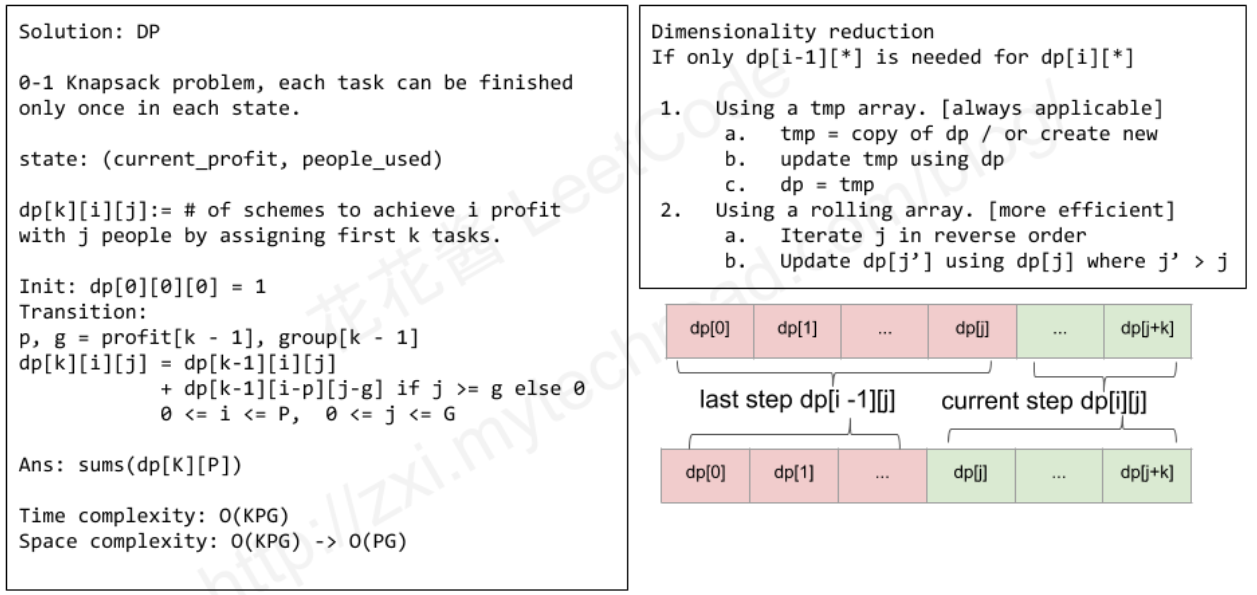
\includegraphics[width=.9\linewidth]{./pic/crime.png}

\begin{itemize}
\item 题目中说了结果可能非常大,要对一个超大数取余,看到这里,我们也就该明白为了不爆栈,只能用动态规划 Dynamic Programming 来做,LeetCode 里有好多题都是要对这个 1e9+7 取余,不知道为啥都是对这个数取余。Anyway,who cares,还是来想想 dp 数组如何定义以及怎么推导状态转移方程吧。
\end{itemize}

首先来看分配黑帮资源时候都需要考虑哪些因素,总共有三点,要干几票买卖,要用多少人,能挣多少钱。所以我们需要一个三维的 dp 数组,其中 dp[k][i][j] 表示最多干k票买卖,总共用了i个人,获得利润为j的情况下分配方案的总数,初始化 dp\footnotemark[2]{}\textsuperscript{,}\,\footnotemark[2]{}\textsuperscript{,}\,\footnotemark[2]{} 为1。

现在来推导状态转移方程,整个规划的核心是买卖,总共买卖的个数是固定的,每多干一票买卖,可能的分配方法就可能增加,但不可能减少的,因为假如当前已经算出来做 k-1 次买卖的分配方法总数,再做一次买卖,之前的分配方法不会减少,顶多是人数不够,做不成当前这票买卖而已,所以我们的 dp[k][i][j] 可以先更新为 dp[k-1][i][j],然后再来看这第k个买卖还能不能做,我们知道假设这第k个买卖需要g个人,能获得利润p,只有当我们现在的人数i大于等于g的时候,才有可能做这个任务,我们要用g个人来做任务k的话,那么其余的 k-1 个任务只能由 i-g 个人来做了,而且由于整个需要产生利润j,第k个任务能产生利润p,所以其余的 k-1 个任务需要产生利润 j-p,由于利润不能是负值,所以我们还需要跟0比较,取二者的最大值

综上所述,若我们选择做任务k,则能新产生的分配方案的个数为 dp[k-1][i-g][max(0,j-p)],记得每次累加完要对超大数取余。最终我们需要将 dp[n][i][P] ( 0 <= i <= G ) 累加起来,因为我们不一定要全部使用G个人,只要能产生P的利润,用几个人都没关系,而k是表示最多干的买卖数,可能上并没有干到这么多,所以只需要累加人数这个维度即可,

\begin{minted}[frame=lines,fontsize=\scriptsize,linenos=false]{java}
public int profitableSchemes(int n, int minProfit, int[] group, int[] profit) { // 0-1背包问题:每场罪恶在每个状态里最多只能存在一次
    int mod = (int)1e9 + 7, ans = 0;
    int m = group.length;
    int [][][] dp = new int [m+1][n+1][minProfit + 1]; 
    dp[0][0][0] = 1;
    for (int k = 1; k <= m; k++) {
        int p = profit[k-1], g = group[k-1];
        for (int i = 0; i <= n; i++) 
            for (int j = 0; j <= minProfit; j++) {
                dp[k][i][j] = dp[k-1][i][j];
                if (i >= g)
                    dp[k][i][j] = (dp[k][i][j] + dp[k-1][i-g][Math.max(0, j-p)]) % mod;
            }
    }
    for (int i = 0; i <= n; i++) 
        ans = (ans + dp[m][i][minProfit]) % mod;
    return ans;
}
\end{minted}
\subsection{优化一下空间复杂度: 二维dp Dimension reduction by using rolling array.}
\label{sec-1-26-2}

因为当前做的第k个任务,只跟前 k-1 个任务的分配方案有关,所以并不需要保存所有的任务个数的分配方式。这样我们就节省了一个维度,但是需要注意的是,更新的时候i和j只能从大到小更新,这个其实也不难理解,因为此时 dp[i][j] 存的是前 k-1 个任务的分配方式,所以更新第k个任务的时候,一定要从后面开始覆盖,因为用到了前面的值,若从前面的值开始更新的话,就不能保证用到的都是前 k-1 个任务的分配方式,有可能用到的是已经更新过的值,就会出错.
\begin{minted}[frame=lines,fontsize=\scriptsize,linenos=false]{java}
public int profitableSchemes(int n, int minProfit, int[] group, int[] profit) { // 0-1背包问题:每场罪恶在每个状态里最多只能存在一次
    int mod = (int)1e9 + 7, ans = 0;
    int m = group.length;
    int [][] dp = new int [n+1][minProfit + 1]; 
    dp[0][0] = 1;
    for (int k = 1; k <= m; k++) {
        int p = profit[k-1], g = group[k-1];
        for (int i = n; i >= g; i--)  // i >= 
            for (int j = minProfit; j >= 0; j--) 
                dp[i][j] = (dp[i][j] + dp[i-g][Math.max(0, j-p)]) % mod; // 保证了这一行覆盖原数组的正确性
    }
    for (int i = 0; i <= n; i++) 
        ans = (ans + dp[i][minProfit]) % mod;
    return ans;
}
\end{minted}
\subsection{递归 + 记忆数组来做 todo: 改天补上}
\label{sec-1-26-3}

基本思想跟解法一没有太大的区别,递归的记忆数组其实跟迭代形式的 dp 数组没有太大的区别,作用都是保存中间状态从而减少大量的重复计算。这里稍稍需要注意下的就是递归函数中的 corner case,当 k=0 时,则根据j的值来返回0或1,当j小于等于0,返回1,否则返回0,相当于修改了初始化值(之前都初始化为了整型最小值),然后当j小于0时,则j赋值为0,因为利润不能为负值。然后就看若当前的 memo[k][i][j] 已经计算过了,则直接返回即可,
\begin{itemize}
\item \url{https://www.cnblogs.com/grandyang/p/11108205.html}
\end{itemize}

\section{377. Combination Sum IV 没能认出这个题目是考DP}
\label{sec-1-27}
Given an array of distinct integers nums and a target integer target, return the number of possible combinations that add up to target.
The answer is guaranteed to fit in a 32-bit integer.
\begin{minted}[frame=lines,fontsize=\scriptsize,linenos=false]{java}
public int combinationSum4(int[] nums, int target) {
    int n = nums.length;
    int [] dp = new int [target +1 ];
    dp [0] = 1;
    for (int i = 1; i <= target; i++) {
        for (int j = 0; j < n; j++) {
            if (i - nums[j] >= 0)
                dp[i] += dp[i-nums[j]];
        }
    }
    return dp[target];
}
\end{minted}

\section{1049. Last Stone Weight II}
\label{sec-1-28}
You are given an array of integers stones where stones[i] is the weight of the ith stone.
We are playing a game with the stones. On each turn, we choose any two stones and smash them together. Suppose the stones have weights x and y with x <= y. The result of this smash is:
If x \texttt{= y, both stones are destroyed, and
If x !} y, the stone of weight x is destroyed, and the stone of weight y has new weight y - x.
At the end of the game, there is at most one stone left.
Return the smallest possible weight of the left stone. If there are no stones left, return 0.
\begin{minted}[frame=lines,fontsize=\scriptsize,linenos=false]{java}
public int lastStoneWeightII(int[] stones) {
    int n = stones.length;
    int sum = Arrays.stream(stones).sum();
    boolean[] dp = new boolean[sum+1];
    dp[0] = true;
    sum = 0;
    for (int v : stones) {
        sum += v;
        for (int i = sum; i >= v; i--) 
            if (dp[i-v]) dp[i] = true;
    }
    for (int i = sum/2; i >= 0; i--) 
        if (dp[i]) return sum - i * 2;
    return 0;
}
\end{minted}

\section{1449. Form Largest Integer With Digits That Add up to Target}
\label{sec-1-29}
Given an array of integers cost and an integer target. Return the maximum integer you can paint under the following rules:
The cost of painting a digit (i+1) is given by cost[i] (0 indexed).
The total cost used must be equal to target.
Integer does not have digits 0.
Since the answer may be too large, return it as string.
If there is no way to paint any integer given the condition, return "0".
\begin{minted}[frame=lines,fontsize=\scriptsize,linenos=false]{java}
public String largestNumber(int[] cost, int target) { 
    int n = cost.length;
    int [] dp = new int [target+1];
    Arrays.fill(dp, -1);
    dp[0] = 0;
    for (int i = 0; i < n; i++) {
        for (int j = cost[i]; j <= target; j++) {
            if (dp[j-cost[i]] >= 0)
                dp[j] = Math.max(dp[j], dp[j-cost[i]]+1);
        }
    }
    if (dp[target] < 0) return "0";
    char [] ans = new char[dp[target]]; // 采樱桃机器人数组路线那天可以想出来,今天这个路径居然没有想出来!
    int left = target;
    for (int i = 0; i < dp[target]; i++) {
        for (int j = n; j > 0; j--) {
            if (left >= cost[j-1] && dp[left] == dp[left-cost[j-1]] + 1) {
                ans[i] = (char)('0' + j);
                left -= cost[j-1];
                break;
            }
        }
    }
    return String.valueOf(ans);
}
\end{minted}

\section{516. Longest Palindromic Subsequence}
\label{sec-1-30}
Given a string s, find the longest palindromic subsequence's length in s.
A subsequence is a sequence that can be derived from another sequence by deleting some or no elements without changing the order of the remaining elements.
\begin{minted}[frame=lines,fontsize=\scriptsize,linenos=false]{java}
 public int longestPalindromeSubseq(String s) {
    int n = s.length();
    int [][] dp = new int [n][n];
    dp[n-1][n-1] = 1;
    for (int i = n-2; i >= 0; i--) {
        dp[i][i] = 1;
        for (int j = i+1; j < n; j++) {
            if (s.charAt(i) == s.charAt(j))
                dp[i][j] = 2 + dp[i+1][j-1];
            else dp[i][j] = Math.max(dp[i+1][j], dp[i][j-1]);
        }
    }
    return dp[0][n-1];
}
\end{minted}

\section{1143. Longest Common Subsequence}
\label{sec-1-31}
Given two strings text1 and text2, return the length of their longest common subsequence. If there is no common subsequence, return 0.
A subsequence of a string is a new string generated from the original string with some characters (can be none) deleted without changing the relative order of the remaining characters.
For example, "ace" is a subsequence of "abcde".
A common subsequence of two strings is a subsequence that is common to both strings.
\begin{minted}[frame=lines,fontsize=\scriptsize,linenos=false]{java}
public int longestCommonSubsequence(String S, String T) {
    int m = S.length();
    int n = T.length();
    int [][] dp = new int [m+1][n+1];
    for (int i = 1; i <= m; i++) 
        for (int j = 1; j <= n; j++) 
            if (S.charAt(i-1) == T.charAt(j-1)) dp[i][j] = dp[i-1][j-1] + 1;
            else dp[i][j] = Math.max(dp[i-1][j], dp[i][j-1]);
    return dp[m][n];
}
\end{minted}

\section{1092. Shortest Common Supersequence - Hard}
\label{sec-1-32}
Given two strings str1 and str2, return the shortest string that has both str1 and str2 as subsequences. If there are multiple valid strings, return any of them.

A string s is a subsequence of string t if deleting some number of characters from t (possibly 0) results in the string s.
\begin{itemize}
\item 参考的标准答案:
\end{itemize}
\begin{minted}[frame=lines,fontsize=\scriptsize,linenos=false]{java}
public void longestCommonSubsequence(String S, String T) { // 标准模板,记住
    int m = S.length();
    int n = T.length();
    for (int i = 1; i <= m; i++) 
        for (int j = 1; j <= n; j++) 
            if (S.charAt(i-1) == T.charAt(j-1)) dp[i][j] = dp[i-1][j-1] + 1;
            else dp[i][j] = Math.max(dp[i-1][j], dp[i][j-1]);
}
int [][] dp;
public String shortestCommonSupersequence(String s, String t) {
    int m = s.length();
    int n = t.length();
    dp = new int [m+1][n+1];
    longestCommonSubsequence(s, t); // fill dp table
    int i = m, j = n;
    StringBuilder sb = new StringBuilder();
    while (i-1 >= 0 && j-1 >= 0) {
        if (s.charAt(i-1) == t.charAt(j-1)) {
            sb.append(s.charAt(i-1));
            --i;
            --j;
        } else {
            if (dp[i][j] == dp[i-1][j]) {
                sb.append(s.charAt(i-1));
                --i;
            } else {
                sb.append(t.charAt(j-1));
                --j;
            }
        }
    }
    if (i > 0) sb.append((new StringBuilder(s.substring(0, i))).reverse());
    if (j > 0) sb.append((new StringBuilder(t.substring(0, j))).reverse());
    return sb.reverse().toString();
}
\end{minted}
\begin{itemize}
\item 自己写的
\end{itemize}
\begin{minted}[frame=lines,fontsize=\scriptsize,linenos=false]{java}
public String getLongestCommonSubsequence(String S, String T) { // 标准模板,记住
    int m = S.length();
    int n = T.length();
    int [][] dp = new int [m+1][n+1];
    for (int i = 1; i <= m; i++) 
        for (int j = 1; j <= n; j++) 
            if (S.charAt(i-1) == T.charAt(j-1)) dp[i][j] = dp[i-1][j-1] + 1;
            else dp[i][j] = Math.max(dp[i-1][j], dp[i][j-1]);
    int i = m, j = n;
    StringBuilder sb = new StringBuilder();
    while (i-1 >= 0 && j-1 >= 0) {
        if (S.charAt(i-1) == T.charAt(j-1)) {
            sb.insert(0, S.charAt(i-1));
            --i;
            --j;
        } else {
            if (dp[i-1][j] >= dp[i][j-1]) --i;
            else --j;
        }
    }
    return sb.toString();
}
public String shortestCommonSupersequence(String s, String t) {
    int m = s.length();
    int n = t.length();
    int i = 0, j = 0;
    String sub = getLongestCommonSubsequence(s, t);
    String res = "";
    for (char c : sub.toCharArray()) {
        while (s.charAt(i) != c) {
            res += s.charAt(i);
            i++;
        }
        while (t.charAt(j) != c) {
            res += t.charAt(j);
            j++;
        }
        res += c;
        i++;
        j++;
    }
    return res + s.substring(i) + t.substring(j);
}
\end{minted}
\section{546. Remove Boxes - Hard}
\label{sec-1-33}
You are given several boxes with different colors represented by different positive numbers.

You may experience several rounds to remove boxes until there is no box left. Each time you can choose some continuous boxes with the same color (i.e., composed of k boxes, k >= 1), remove them and get k * k points.

Return the maximum points you can get.
\begin{minted}[frame=lines,fontsize=\scriptsize,linenos=false]{java}
// 定义dp[l][r][k]表示在[l, r]区间并且在后面包含了k个与boxes[r]相同颜色的boxes的情况下,可以获得的最大得分,显然题目要求的就是dp[0][boxes.size() - 1][0]。
// 首先将dp[l][r][k]的值初始化为dp[l][r - 1][0] + (k + 1)^2,表示首先消除l到r-1之间的boxes,然后将boxes[r]连同后面的k个boxes一起消除。
// 然后就尝试对dp[l][r][k]进行更新了:
// 如果在l到r-1区间内有boxes[i]和boxes[r]相同的字符,那么可以尝试首先将区间[i + 1, r - 1]消除,这样i就和后面的k + 1个boxes连起来了,
// 其可以获得分数就是需要进一步计算的dp[l][i][k + 1]。
private int dfs(int [] arr, int i, int j, int  k) {
    if (i > j) return 0;
    if (dp[i][j][k] > 0) return dp[i][j][k];
    int res = dfs(arr, i, j-1, 0) + (k+1)*(k+1);
    for (int x = i; x < j; x++) 
        if (arr[x] == arr[j]) {
            res = Math.max(res, dfs(arr, i, x, k+1) + dfs(arr, x+1, j-1, 0));
        }
    return dp[i][j][k] = res;
}
int [][][] dp;
int n;
public int removeBoxes(int[] boxes) {
    n = boxes.length;
    dp = new int [n][n][n];
    return dfs(boxes, 0, n-1, 0);
}
\end{minted}
\section{1531. String Compression II - Hard}
\label{sec-1-34}
Run-length encoding is a string compression method that works by replacing consecutive identical characters (repeated 2 or more times) with the concatenation of the character and the number marking the count of the characters (length of the run). For example, to compress the string "aabccc" we replace "aa" by "a2" and replace "ccc" by "c3". Thus the compressed string becomes "a2bc3".

Notice that in this problem, we are not adding '1' after single characters.

Given a string s and an integer k. You need to delete at most k characters from s such that the run-length encoded version of s has minimum length.

Find the minimum length of the run-length encoded version of s after deleting at most k characters.
\begin{minted}[frame=lines,fontsize=\scriptsize,linenos=false]{java}
 private int dfs(char [] s, int idx, int cnt) { // 求从下标index开始向后,所有长度为count的子序列中,编码后的最小长度
    if (cnt == 0) return 0;
    if (idx == n) return Integer.MAX_VALUE;   // 当下标越界时还未找到长度为count的子序列
    if (dp[idx][cnt] > 0) return dp[idx][cnt];
    int min = Integer.MAX_VALUE, leftCnt = 0;
    boolean [] vis = new boolean [26];
    for (int i = idx; i < n; i++) {
        if (vis[s[i]-'a']) continue;   // 优化:已处理过当前的字母,跳过
        if (idx > 0 && s[i] == s[idx-1]) continue;
        vis[s[i]-'a'] = true;
        leftCnt = 0;
        for (int j = i; j < n; j++) {
            if (s[j] != s[i]) continue;
            leftCnt++;
            if (cnt - leftCnt < 0) break;  // 如果左半部分长度大于子序列长度,退出
            int right = dfs(s, j+1, cnt - leftCnt);
            if (right == Integer.MAX_VALUE) continue;
            int left = String.valueOf(leftCnt).length();
            min = Math.min(min, left + right + (left == 1 && leftCnt == 1 ? 0 : 1));
        }
    }
    return dp[idx][cnt] = min;
}
int [][] dp;
int n;
public int getLengthOfOptimalCompression(String s, int k) {
    n = s.length();
    dp = new int [n][n-k+1];
    return dfs(s.toCharArray(), 0, n-k);
}
\end{minted}
\subsection{决策类DP总结}
\label{sec-1-34-1}
\begin{itemize}
\item \url{https://leetcode-cn.com/problems/string-compression-ii/solution/jie-ti-si-kao-guo-cheng-yu-jie-fa-zong-jie-by-ruit/}
\end{itemize}

\section{1000. Minimum Cost to Merge Stones}
\label{sec-1-35}
There are n piles of stones arranged in a row. The ith pile has stones[i] stones.
A move consists of merging exactly k consecutive piles into one pile, and the cost of this move is equal to the total number of stones in these k piles.
Return the minimum cost to merge all piles of stones into one pile. If it is impossible, return -1.
\begin{minted}[frame=lines,fontsize=\scriptsize,linenos=false]{java}
public int mergeStones(int[] stones, int k) {
    int n = stones.length;
    if ((n-1) % (k-1) != 0) return -1;
    int [][] dp = new int[n][n];
    int [] pre = new int[n+1];
    for (int i = 1; i <= n; i++) 
        pre[i] = pre[i-1] + stones[i-1];
    int j = 0;
    for (int len = k; len <= n; len++) {
        for (int i = 0; i+len-1 < n; i++) {
            j = i + len -1;
            dp[i][j] = Integer.MAX_VALUE; // have to initialize it here !!!
            for (int x = i; x < j; x += k-1) 
                dp[i][j] = Math.min(dp[i][j], dp[i][x] + dp[x+1][j]);
            if ((j - i) % (k - 1) == 0) // 如果总长度满足合并只剩一个数的条件,则可以再合并一次
                dp[i][j] += pre[j+1] - pre[i];
        }
    }
    return dp[0][n-1];
}
\end{minted}

\section{1039. Minimum Score Triangulation of Polygon}
\label{sec-1-36}
You have a convex n-sided polygon where each vertex has an integer value. You are given an integer array values where values[i] is the value of the ith vertex (i.e., clockwise order).
You will triangulate the polygon into n - 2 triangles. For each triangle, the value of that triangle is the product of the values of its vertices, and the total score of the triangulation is the sum of these values over all n - 2 triangles in the triangulation.
Return the smallest possible total score that you can achieve with some triangulation of the polygon.
\begin{minted}[frame=lines,fontsize=\scriptsize,linenos=false]{java}
// 动态规划,递归可以使逻辑简单(本质还是动态规划)将多边形起
// 始位置设为start,end, 用一个数组dp来记录任意起始位置的score
// 为了计算dp[start][end], 我们用一个index k在start到end之间遍
// 历dp[start][end] = min(dp[start][k] + dp[k][end] + A[start]
// * A[k] * A[end])结果为dp[0][n - 1]注意:相邻的dp[i][i + 1]
// = 0, 因为两条边无法组成三角形
private int dfs(int [] arr, int x, int y) {
    if (y - x < 2) return dp[x][y] = 0;
    if (dp[x][y] > 0) return dp[x][y];
    int min = Integer.MAX_VALUE;
    for (int i = x+1; i < y; i++) 
        min = Math.min(min, dfs(arr, x,  i) + dfs(arr, i, y) + arr[x]*arr[i]*arr[y]);
    return dp[x][y] = min;
}
int [][] dp;
int n;
public int minScoreTriangulation(int[] arr) {
    n = arr.length;
    dp = new int [n][n];
    return dfs(arr, 0, n-1);
}
\end{minted}

\section{375. Guess Number Higher or Lower II - Medium}
\label{sec-1-37}
We are playing the Guessing Game. The game will work as follows:

I pick a number between 1 and n.

You guess a number.

If you guess the right number, you win the game.

If you guess the wrong number, then I will tell you whether the number I picked is higher or lower, and you will continue guessing.

Every time you guess a wrong number x, you will pay x dollars. If you run out of money, you lose the game.

Given a particular n, return the minimum amount of money you need to guarantee a win regardless of what number I pick.

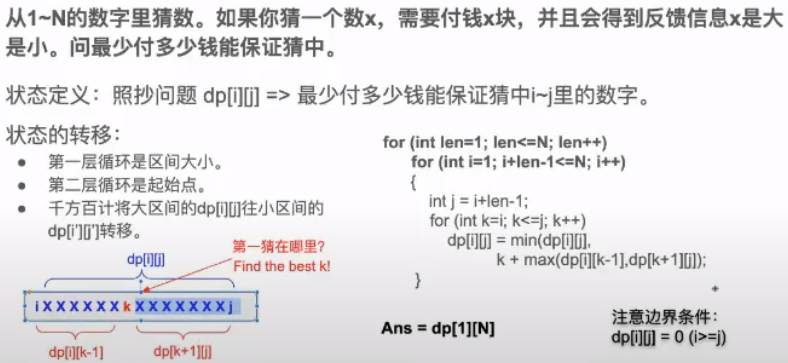
\includegraphics[width=.9\linewidth]{./pic/guessNumber.png}

\begin{minted}[frame=lines,fontsize=\scriptsize,linenos=false]{java}
private int dfs(int l, int r) {
    if (dp[l][r] > 0) return dp[l][r];
    if (l == r) return dp[l][r] = 0;
    if (l == r-1) return dp[l][r] = Math.min(l, r);
    int min = Integer.MAX_VALUE;
    for (int i = l; i <= r; i++) 
        min = Math.min(min, i + Math.max((i == r ? i : dfs(i+1, r)), (i == l ? i : dfs(l, i-1))));
    return dp[l][r] = min;
}
int [][] dp;
public int getMoneyAmount(int n) {
    dp = new int[n+1][n+1];
    return dfs(1, n);
}
\end{minted}
\section{1478. Allocate Mailboxes - Hard}
\label{sec-1-38}
Given the array houses and an integer k. where houses[i] is the location of the ith house along a street, your task is to allocate k mailboxes in the street.

Return the minimum total distance between each house and its nearest mailbox.

The answer is guaranteed to fit in a 32-bit signed integer.

解题思路分析:

对于如何安排邮箱位置,看到很多文章说应放在中位数的位置上,比如一共有1,2,3,4这4间房屋,不论房屋间的距离是多少,如果只有一个邮箱的话,放在房间2处(3也可以)最为合理。这个说法虽然正确,但实际上并不恰当。我们简单的讨论一下这个问题:
\begin{minted}[frame=lines,fontsize=\scriptsize,linenos=false]{java}
1.当只有1栋房屋,1个邮箱时,显然将邮箱放在房屋处最为合理,这时邮箱与房屋的距离为0。
2.当有2栋房屋,1个邮箱时,比如房屋1在坐标0处,房屋2在坐标10处,此时如果将邮箱放在坐标0的话,它与两栋房屋的距离和为10。
  放在坐标10的情况下距离和也为10。另外我们可以看出,不论邮箱放在两栋房屋之间的任意位置上,它与房屋的距离和都是10。因此
  通过此例可得出,中位数的说法虽然正确,但并不全面,不过这不影响本题解题,对于本题,我们统一将邮箱安排在房屋位置上是为
  了方便计算,因此才得出中位数的说法(本例房屋1和2都可以看做是中位数)。
3.当有3栋房屋,1个邮箱时,此时通过上面的例子可知,对于两侧的房子,将邮筒放在他们之间的任何位置对于结果没有任何影响,距
  离和都是两栋房子间的距离。但邮箱的位置会对中间的房子产生影响,因此,将其放置在中间房子的坐标上最为合理,这样邮箱与中
  间房屋的距离为0,可使得全局总距离最小。而中间的房屋正是3个房屋的中位数。
4.当有4栋房屋,1个邮箱时,与上例同理,对于两侧的房子,将邮筒放在他们之间的任何位置对于结果没有任何影响,因此邮箱可以考
  虑放在中间两个房屋的任何一个位置上。另外对于中间两个房屋,不论邮箱放置在其任何一个位置上,对于总距离都不会产生影响
 (这相当于第2条)。
\end{minted}

因此我们可以得出结论,当有N栋房屋,1个邮箱时,我们将邮箱放在房屋下标的中位数上最为合理。那么,如果有多个邮箱时该怎么办?其实也不难,本题最终可以理解为,我们将一个房屋数组分割为K个子数组(k为邮筒个数),每一个子数组中放置一个邮筒,求最优分割方式。这就变为了经典的动态规划DP问题,对于DP问题我习惯采用递归加记忆数组的方式,本题我们也采用递归方式讲解。

首先建立一个递归函数,参数为当前子区间开始位置index,以及剩余未分配邮筒个数k。起始时,子区间开始位置为下标0,邮筒个数为题目给定的整数k。递归时,当前子区间的开始坐标是参数index,结束坐标范围理论上可以是当前index到数组末尾为止,不过这里有一处可以优化,即要保证剩下的k-1个邮筒都能分配出去的话,还需要至少k-1个子区间,也就是说除了当前子区间外还至少需要k-1个房屋,因此当前子区间的结束坐标范围应该是当前index到length-k为止。我们从index循环至length-k,分别作为当前子区间的结束位置end。并通过中位数方式求出当前子区间[index, end]放置邮筒后的距离和(后文会给出方法)。然后将end加一作为下一个子区间的开始位置,同时k值减去一作为参数传入递归子问题中继续求解。递归函数的返回值加上当前子区间的距离和即是选择当前子区间范围后的一个结果sum。循环完所有当前子区间的结束位置end之后,所有sum中的最小值即是最优方案,也是本层递归的返回值。

接下来再为递归加上一个记忆数组。记忆数组相当于动态规划中使用到的DP数组。由于递归函数中存在2个变量,因此我们需要使用一个2维数组来描述该递归函数,并记录它的返回值。

最后,上文中提到需要求解子区间内放置一个邮筒后所有房屋与邮筒的距离和。这个问题没有太好的方式,只能暴力累加每个房屋与中位数房屋所在位置的距离。为了提高效率,我们可以事先计算好所有区间(排列组合)内放置一个邮筒时的距离和,方便递归中使用,也避免重复运算。这里可能有人会提出质疑,既然递归方法中已经使用了记忆数组,目的就是防止重复计算,这里为什么还担心重复计算距离和呢?原因很简单,记忆数组是二维数组,即在两个条件都满足的情况下才会使用记忆数组中的数据,比如我们计算过以下标5作为子区间起点,并且当前还剩2个油桶的递归函数返回值为x,即memo\footnote{DEFINITION NOT FOUND.}\textsuperscript{,}\,\footnote{DEFINITION NOT FOUND.}=x,再次遇到相同问题时我们可以直接返回x。但是遇到memo\footnotemark[4]{}\textsuperscript{,}\,\footnotemark[3]{}或者memo\footnotemark[4]{}\textsuperscript{,}\,\footnotemark[1]{}时,我们尚未做出过计算,同样还会进入到递归函数内部,如果没有事前计算好下标5到end(end取值范围是5到length-k)的距离和的话,还要重复计算一遍。

对于上述问题,还有一个更好的优化方式即再建立一个保存距离和的记忆数组,计算一个距离和记录一个,方便下次使用。

\begin{minted}[frame=lines,fontsize=\scriptsize,linenos=false]{java}
private int getDist(int [] arr, int i, int j) { // 求区间start到end间放置邮筒后的距离和 i: left, j: right
    if (dist[i][j] > 0) return dist[i][j];
    int m = i + (j-i)/2, v = arr[m], sum = 0;
    for (int k = i; k <= j; k++) 
        sum += Math.abs(arr[k] - v);
    return dist[i][j] = sum;
}
private int dfs(int [] arr, int idx, int k) {  // idx: 待分割大子区间的起始坐标;k: 待分割成的子区间的个数 
    if (idx == n || idx == n-k) return 0;
    if (dp[idx][k] > 0) return dp[idx][k];
    if (k == 1) return dp[idx][k] = getDist(arr, idx, n-1);
    int res = Integer.MAX_VALUE;
    for (int i = idx; i < n-(k-1); i++) 
        res = Math.min(res, getDist(arr, idx, i) + dfs(arr, i+1, k-1));
    return dp[idx][k] = res;
}
int [][] dp;
int [][] dist; // 这也是一种记忆数组优化
int n;
public int minDistance(int [] houses, int k) {
    n = houses.length;
    dist = new int [n][n];
    dp = new int [n][k+1];
    Arrays.sort(houses);
    return dfs(houses, 0, k);
}
\end{minted}

\section{486. Predict the Winner}
\label{sec-1-39}
You are given an integer array nums. Two players are playing a game with this array: player 1 and player 2.
Player 1 and player 2 take turns, with player 1 starting first. Both players start the game with a score of 0. At each turn, the player takes one of the numbers from either end of the array (i.e., nums\footnotemark[2]{} or nums[nums.length - 1]) which reduces the size of the array by 1. The player adds the chosen number to their score. The game ends when there are no more elements in the array.
Return true if Player 1 can win the game. If the scores of both players are equal, then player 1 is still the winner, and you should also return true. You may assume that both players are playing optimally.

博弈类题目,使用minMax思想,使自己分数最大化,对手分数尽量小,递归自顶向下求解。

该题不使用备忘机制同样能通过测试例,只不过耗时相对较长,单纯的比较取数后两players的分数差即可:Math.max(nums[l] - getScore(nums, l + 1, r), nums[r] - getScore(nums, l, r - 1));

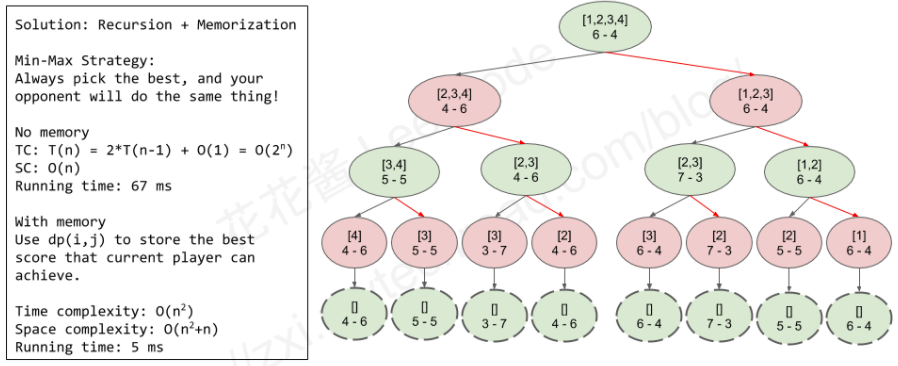
\includegraphics[width=.9\linewidth]{./pic/predictWinner.png}

\begin{minted}[frame=lines,fontsize=\scriptsize,linenos=false]{java}
private int helper( int [] arr, int i, int j) {
    if (i == j) return arr[i];
    else return Math.max(arr[i] - helper(arr, i+1, j), arr[j] - helper(arr, i, j-1));
}
public boolean PredictTheWinner(int[] nums) {
    int n = nums.length;
    if (n == 1) return true;
    return helper(nums, 0, n-1) >= 0;
}
\end{minted}

\section{877. Stone Game}
\label{sec-1-40}
Alice and Bob play a game with piles of stones. There are an even number of piles arranged in a row, and each pile has a positive integer number of stones piles[i].
The objective of the game is to end with the most stones. The total number of stones across all the piles is odd, so there are no ties.
Alice and Bob take turns, with Alice starting first. Each turn, a player takes the entire pile of stones either from the beginning or from the end of the row. This continues until there are no more piles left, at which point the person with the most stones wins.
Assuming Alice and Bob play optimally, return true if Alice wins the game, or false if Bob wins.
\begin{minted}[frame=lines,fontsize=\scriptsize,linenos=false]{java}
// 使用helper函数表示Alex能比Lee多选的分数。可能比双函数更简洁易懂了。
// 记忆化递归的缺点:1.有可能爆栈;2.无法降维,而DP是可以降维的。
// 模板:
// dfs + memoization模板
private int dfs(int [] arr, int l, int r) {
    if (l > r) return 0;
    if (dp[l][r] > 0) return dp[l][r]; // 走了来时的路,不需要重走,直接返回
    dp[l][r] = Math.max(arr[l] - dfs(arr, l+1, r), arr[r]-dfs(arr, l, r-1));
    return dp[l][r];
}
int [][] dp; 
public boolean stoneGame(int[] piles) {
    int n = piles.length;
    dp = new int[n][n];
    return dfs(piles, 0, n-1) > 0;
}
// 动态规划解法比较难想,dp数组的第i个位置表示的是从第i个石头到第i+l-1个石头之间最大的比对手得分。
// 使用的是一个长度变量和起始索引,计算每个位置开始的长度1~N长度的区间的dp状态。
public boolean stoneGame(int[] piles) {
    int n = piles.length;
    int [][] dp = new int[n][n];
    for (int i = n-1; i >= 0; i--) { // 最后一列
        dp[i][i] = piles[i];         // 填右上角
        for (int j = i+1; j < n; j++) 
            dp[i][j] = Math.max(piles[i] - dp[i+1][j], piles[j]-dp[i][j-1]);

    }
    return dp[0][n-1] > 0;
}
\end{minted}
\section{1140. Stone Game II}
\label{sec-1-41}
Alice and Bob continue their games with piles of stones.  There are a number of piles arranged in a row, and each pile has a positive integer number of stones piles[i].  The objective of the game is to end with the most stones. 
Alice and Bob take turns, with Alice starting first.  Initially, M = 1.
On each player's turn, that player can take all the stones in the first X remaining piles, where 1 <= X <= 2M.  Then, we set M = max(M, X).
The game continues until all the stones have been taken.
Assuming Alice and Bob play optimally, return the maximum number of stones Alice can get.
\begin{minted}[frame=lines,fontsize=\scriptsize,linenos=false]{java}
// dfs + memoization模板
// 当次取的最优策略是限制下一次取的数量
private int dfs(int [] arr, int idx, int m) {
    if (dp[idx][m] > 0) return dp[idx][m];
    if (idx == n) return 0;
    if (idx >= n - 2 * m) {
        dp[idx][m] = suf[idx];
        return dp[idx][m];
    }
    int min = Integer.MAX_VALUE;
    for (int i = 1; i <= 2 * m; i++) // 选择限制对手得分最少的情况
        min = Math.min(min, dfs(arr, idx+i, Math.max(m, i))); 
    dp[idx][m] = suf[idx] - min;
    return dp[idx][m];
}
int [][] dp; 
int [] suf;
int n;
public int stoneGameII(int[] piles) {
    n = piles.length;
    dp = new int [n][2*n];
    suf = new int [n+1];
    for (int i = n-1; i >= 0; i--) 
        suf[i] = suf[i+1] + piles[i];
    return dfs(piles, 0, 1);
}
\end{minted}
\section{1872. Stone Game VIII}
\label{sec-1-42}
Alice and Bob take turns playing a game, with Alice starting first.
There are n stones arranged in a row. On each player's turn, while the number of stones is more than one, they will do the following:
Choose an integer x > 1, and remove the leftmost x stones from the row.
Add the sum of the removed stones' values to the player's score.
Place a new stone, whose value is equal to that sum, on the left side of the row.
The game stops when only one stone is left in the row.
The score difference between Alice and Bob is (Alice's score - Bob's score). Alice's goal is to maximize the score difference, and Bob's goal is the minimize the score difference.
Given an integer array stones of length n where stones[i] represents the value of the ith stone from the left, return the score difference between Alice and Bob if they both play optimally.
\begin{minted}[frame=lines,fontsize=\scriptsize,linenos=false]{java}
// 使用 dp(i) 表示还剩下 [i, n) 要选择的情况下,Alice 所能得到的最大分数差。
//     对于某个玩家来说,其对应决策可以分为两种:
//     选取当前数及之前的所有数(等价于 pres[pos],其中 pos 为上个玩家选完后的下个位置),那么 dp[i] = pres[i] - dp[i+1]。
//     这是因为 bob 也会最大化发挥。
//     不选择当前数(可能选下一个,下下一个。。。 etc),那么 dp[i] = dp[i + 1]
public int stoneGameVIII(int[] stones) {
    int n = stones.length;
    int [] dp = new int [n];
    Arrays.fill(dp, Integer.MIN_VALUE);
    int [] pre = new int [n+1];
    for (int i = 1; i <= n; i++)
        pre[i] = pre[i-1] + stones[i-1];
    dp[n-1] = pre[n];
    for (int i = n-2; i >= 0; i--) 
        dp[i] = Math.max(dp[i+1], pre[i+1]-dp[i+1]);
    return dp[1];
}
\end{minted}

\section{123. Best Time to Buy and Sell Stock III}
\label{sec-1-43}
You are given an array prices where prices[i] is the price of a given stock on the ith day.
Find the maximum profit you can achieve. You may complete at most two transactions.
Note: You may not engage in multiple transactions simultaneously (i.e., you must sell the stock before you buy again).
\begin{minted}[frame=lines,fontsize=\scriptsize,linenos=false]{java}
// k 次交易 = k 个 non-overlapping subarray
//     以这个角度去想,无非就是从两个方向扫描,
//     利用 localMin / localMax 与当前元素的差值,去构造从左边/右边扫的 dp 数组。
//     left[i] : 从最左面到 i 所能获得的最大利益(单次交易)
//     right[i] : 从 i 到最右面所能获得的最大利益(单次交易)
public int maxProfit(int[] prices) {
    int n = prices.length;
    int [] left = new int [n];
    int [] right = new int[n];
    int locMin = prices[0];
    int globalMax = Integer.MIN_VALUE;
    for (int i = 1; i < n; i++) {
        globalMax = Math.max(globalMax, Math.max(0, prices[i] - locMin));
        locMin = Math.min(locMin, prices[i]);
        left[i] = globalMax;
    }
    int locMax = prices[n-1];
    globalMax = Integer.MIN_VALUE;
    for (int i = n-2; i >= 0; i--) {
        globalMax = Math.max(globalMax, Math.max(0, locMax - prices[i]));
        locMax = Math.max(locMax, prices[i]);
        right[i] = globalMax;
    }
    globalMax = 0;
    for (int i = 0; i < n-1; i++) 
        globalMax = Math.max(globalMax, left[i] + right[i+1]);
    globalMax = Math.max(globalMax, left[n-1]);
    return globalMax;
}
\end{minted}

\section{188. Best Time to Buy and Sell Stock IV}
\label{sec-1-44}
You are given an integer array prices where prices[i] is the price of a given stock on the ith day, and an integer k.
Find the maximum profit you can achieve. You may complete at most k transactions.
Note: You may not engage in multiple transactions simultaneously (i.e., you must sell the stock before you buy again).
\begin{minted}[frame=lines,fontsize=\scriptsize,linenos=false]{java}
public int maxProfit(int k, int [] prices) {
    if (prices == null || prices.length == 0) return 0;
    int n = prices.length;
    int diff = 0;
    if (k >= n/2) {
        int res = 0;
        for (int i = 1; i < n; i++) {
           diff = prices[i] - prices[i-1];
            if (diff > 0) res += diff;
        }
        return res;
    }
    int [][] locMax = new int [n][k+1];
    int [][] gloMax = new int [n][k+1];
    for (int i = 1; i < n; i++) {
        diff = prices[i] - prices[i-1];
        for (int j = 1; j <= k && j * 2 <= i+1; j++) {
            locMax[i][j] = Math.max(locMax[i-1][j], gloMax[i-1][j-1]) + diff;
            gloMax[i][j] = Math.max(locMax[i][j], gloMax[i-1][j]);
        }
    }
    return gloMax[n-1][k];
}
\end{minted}

\section{714. Best Time to Buy and Sell Stock with Transaction Fee}
\label{sec-1-45}
You are given an array prices where prices[i] is the price of a given stock on the ith day, and an integer fee representing a transaction fee.
Find the maximum profit you can achieve. You may complete as many transactions as you like, but you need to pay the transaction fee for each transaction.
Note: You may not engage in multiple transactions simultaneously (i.e., you must sell the stock before you buy again).
\begin{minted}[frame=lines,fontsize=\scriptsize,linenos=false]{java}
public int maxProfit(int[] prices, int fee) {
    int n = prices.length;
    int [] sold = new int[n];
    int [] hold = new int[n];
    hold[0] = -prices[0];
    for (int i = 1; i < n; i++) {
        sold[i] = Math.max(sold[i-1], hold[i-1]+prices[i]-fee);
        hold[i] = Math.max(hold[i-1], sold[i-1]-prices[i]);
    }
    return sold[n-1];
}
\end{minted}

\section{309. Best Time to Buy and Sell Stock with Cooldown}
\label{sec-1-46}
You are given an array prices where prices[i] is the price of a given stock on the ith day.
Find the maximum profit you can achieve. You may complete as many transactions as you like (i.e., buy one and sell one share of the stock multiple times) with the following restrictions:
After you sell your stock, you cannot buy stock on the next day (i.e., cooldown one day).
Note: You may not engage in multiple transactions simultaneously (i.e., you must sell the stock before you buy again).
\begin{itemize}
\item 感觉自己DP的能力还是太弱,越是这样越需要迎难而上。
\item 这个题和714. Best Time to Buy and Sell Stock with Transaction Fee比较像。做题方法都是使用了两个数组:
\item cash 该天结束手里没有股票的情况下,已经获得的最大收益
\item hold 该天结束手里有股票的情况下,已经获得的最大收益
\item 状态转移方程式这样的:
\begin{itemize}
\item cash[i]代表的是手里没有股票的收益,这种可能性是今天卖了或者啥也没干。max(昨天手里有股票的收益+今天卖股票的收益,昨天手里没有股票的收益), 即max(sell[i - 1], hold[i - 1] + prices[i]);
\item hold[i]代表的是手里有股票的收益,这种可能性是今天买了股票或者啥也没干,今天买股票必须昨天休息。所以为max(今天买股票是前天卖掉股票的收益-今天股票的价格,昨天手里有股票的收益)。即max(hold[i - 1], sell[i - 2] - prices[i])。
\end{itemize}
\item 另外需要注意的是,题目说的是昨天卖了股票的话今天不能买,对于开始的第一天,不可能有卖股票的行为,所以需要做个判断。
\item 该算法的时间复杂度是O(n),空间复杂度是O(n)。
\end{itemize}
\begin{minted}[frame=lines,fontsize=\scriptsize,linenos=false]{java}
public int maxProfit(int[] prices) {
    int n = prices.length;
    int [] sold = new int [n];
    int [] hold = new int [n];
    hold[0] = -prices[0];
    for (int i = 1; i < n; i++) {   // ith: do nothing, selling hold[i-1]
        sold[i] = Math.max((i >= 2 ? sold[i-1] : 0), hold[i-1] + prices[i]); // 今天卖了股票,或者今天什么也没有干
        hold[i] = Math.max(hold[i-1], (i >= 2 ? sold[i-2] : 0) - prices[i]); // 今天买了股票,或者今天什么也没有干
    }
    return Math.max(sold[n-1], hold[n-1]);
}
\end{minted}

\section{673. Number of Longest Increasing Subsequence}
\label{sec-1-47}
Given an integer array nums, return the number of longest increasing subsequences.
Notice that the sequence has to be strictly increasing.
\begin{minted}[frame=lines,fontsize=\scriptsize,linenos=false]{java}
public int findNumberOfLIS(int[] nums) { // dynamic programming
    int n = nums.length;
    int [][] arr = new int[n][2];
    int maxLength = 1;
    for (int i = 0; i < n; i++) 
        Arrays.fill(arr[i], 1);
    for (int i = 0; i < n; i++) {
        for (int j = i+1; j < n; j++) {
            if (nums[j] > nums[i]) {
                if (arr[i][0] + 1 > arr[j][0]) {
                    arr[j][0] = arr[i][0] +1;
                    arr[j][1] = arr[i][1];
                    maxLength = Math.max(maxLength, arr[j][0]);
                } else if (arr[i][0] + 1 == arr[j][0])
                    arr[j][1] += arr[i][1];
            }
         }
    }
    int cnt = 0;
    for (int i = 0; i < n; i++) 
        if (arr[i][0] == maxLength) cnt += arr[i][1];
    return cnt;
}
\end{minted}

\section{1896. Minimum Cost to Change the Final Value of Expression - Hard}
\label{sec-1-48}
You are given a valid boolean expression as a string expression consisting of the characters '1','0','\&' (bitwise AND operator),'|' (bitwise OR operator),'(', and ')'.

For example, "()1|1" and "(1)\&()" are not valid while "1", "(((1))|(0))", and "1|(0\&(1))" are valid expressions.
Return the minimum cost to change the final value of the expression.

For example, if expression = "1|1|(0\&0)\&1", its value is 1|1|(0\&0)\&1 = 1|1|0\&1 = 1|0\&1 = 1\&1 = 1. We want to apply operations so that the new expression evaluates to 0.
The cost of changing the final value of an expression is the number of operations performed on the expression. The types of operations are described as follows:

Turn a '1' into a '0'.
Turn a '0' into a '1'.
Turn a '\&' into a '|'.
Turn a '|' into a '\&'.
Note: '\&' does not take precedence over '|' in the order of calculation. Evaluate parentheses first, then in left-to-right order.
\begin{minted}[frame=lines,fontsize=\scriptsize,linenos=false]{java}
private int [] getMinOperations(int va, int vb, int ca, int cb, char sign) {
    if (sign == '&') {
        if (va == 1 && vb == 1)      // 1&1, 将其中一个1反转为0
            return new int [] {1, Math.min(ca, cb)};
        else if (va == 0 && vb == 0) // 0&0, 将其中一个0反转为1,并将&反转为|
            return new int [] {0, Math.min(ca, cb) + 1};
        else return new int [] {0, 1}; // 1&0, 将&反转为|
    } else {
        if (va == 1 && vb == 1)        // 1|1,将其中一个1反转为0,并将|反转为&
            return new int [] {1, Math.min(ca, cb) + 1};
        else if (va == 0 && vb == 0)   // 0|0,将其中一个0反转为1
            return new int [] {0, Math.min(ca, cb)};
        else return new int [] {1, 1}; // 1|0,将|反转为&
    }
}
public int minOperationsToFlip(String expression) {
    Stack<Integer> res = new Stack<>();
    Stack<Character> sgn = new Stack<>();
    Stack<Integer> cnt = new Stack<>();
    for (char c : expression.toCharArray()) {
        if (c == '(' || c == '&' || c == '|') {
            sgn.push(c);
            continue;
        } else if (c == ')') sgn.pop();
        else {
            res.push((int)(c - '0'));
            cnt.push(1);
        }
        if (res.size() > 1 && sgn.peek() != '(') {
            int [] loc = getMinOperations(res.pop(), res.pop(), cnt.pop(), cnt.pop(), sgn.pop());
            res.push(loc[0]); // expr results
            cnt.push(loc[1]); // min operations
        }
    }
    return cnt.peek();
}
\end{minted}

\section{823. Binary Trees With Factors}
\label{sec-1-49}
Given an array of unique integers, arr, where each integer arr[i] is strictly greater than 1.
We make a binary tree using these integers, and each number may be used for any number of times. Each non-leaf node's value should be equal to the product of the values of its children.
Return the number of binary trees we can make. The answer may be too large so return the answer modulo 109 + 7.
\begin{minted}[frame=lines,fontsize=\scriptsize,linenos=false]{java}
public int numFactoredBinaryTrees(int[] arr) {
    int n = arr.length;
    Arrays.sort(arr);
    Map<Integer, Long> dp = new HashMap<>();
    int mod = 1_000_000_007;
    long res = 0;
    long max = 0;
    for (int i = 0; i < n; i++) {
        dp.put(arr[i], 1l);
        for (int j = 0; j < i; j++) {
            if (arr[i] % arr[j] == 0 && dp.containsKey(arr[i]/arr[j])) {
                max = dp.get(arr[i]) + dp.get(arr[j]) * dp.get(arr[i]/arr[j]);
                dp.put(arr[i], max % mod);
            }
        }
        res += dp.get(arr[i]);
        res %= mod;
    }
    return (int)(res % mod);
}
\end{minted}

\section{907. Sum of Subarray Minimums}
\label{sec-1-50}
Given an array of integers arr, find the sum of min(b), where b ranges over every (contiguous) subarray of arr. Since the answer may be large, return the answer modulo 109 + 7.
\begin{minted}[frame=lines,fontsize=\scriptsize,linenos=false]{java}
public int sumSubarrayMins(int[] arr) {
    int n = arr.length;
    // for each A[i], find k <= i <= j, so that A[i] is the min from [k,j]
    // sum += A[i] * (i-k+1) * (j-i+1)
    // so we need to find the next min to the right and to the left
    //这个过程可以简化为使用一个栈。对于被某个数从栈中弹出的数而言,它右侧第一个比它小的数就是这个数。所以我们可以对所有被弹出的数得到左侧的区间范围和右侧的区间范围。我觉得这是一种非常聪明的做法。 这个栈我看得稀里糊涂,再想一下
    long [] right = new long [n];  // next smaller element index to the right 
    long [] left = new long[n];    // next smaller element index to the left
    Stack<Integer> s = new Stack<>();
    for (int i = 0; i < n; i++) {
        while (!s.isEmpty() && arr[i] <= arr[s.peek()]) {
            right[s.pop()] = i-1;
        }
        s.push(i);
    }
    while (!s.isEmpty()) {
        right[s.pop()] = n-1;
    }
    s.clear();
    for (int i = n-1; i >= 0; i--) {
        while (!s.isEmpty() && arr[i] < arr[s.peek()])
            left[s.pop()] = i+1;
        s.push(i);
    }
    while (!s.isEmpty())
        left[s.pop()] = 0;
    long sum = 0;
    long leftsize = 0, rightsize = 0;
    for (int i = 0; i < n; i++) {
        leftsize = i - left[i] +1;
        rightsize = right[i] - i + 1;
        sum += arr[i] * leftsize * rightsize;
        sum %= mod;
    }
    return (int)sum;
}
int mod = 1_000_000_007;
public int sumSubarrayMins(int[] arr) {
    int n = arr.length;
    long [] left = new long[n];
    long [] right = new long[n];
    long sum = 0;
    long cnt = 0;
    int j = 0;
    for (int i = 0; i < n; i++) { // 计算左边比自身大的数的个数
        cnt = 1;
        j = i-1;
        while (j >= 0 && arr[j] >= arr[i]) {
            cnt += left[j];
            j -= left[j];
        }
        left[i] = cnt;
    }
    // 就是因为计算了两个方向,所以对于数组里面有相同元素的情况下,需要特别考虑一下。
    //     不能重复计算, 也不能漏掉,
    //     具体就是一个方向的时候用<=, 另外一个方向的时候用<。 这个在做的时候也bug了。
    for (int i = n-1; i >= 0; i--) { // 计算右边比自身大的数的个数
        cnt = 1;
        j = i+1;
        while (j < n && arr[j] > arr[i]) {
            cnt += right[j];
            j += right[j];
        }
        right [i] = cnt;
    }
    for (int i = 0; i < n; i++) 
        sum += arr[i] * left[i] * right[i];
    return (int) (sum % mod);
}
\end{minted}

\section{494. Target Sum - Medium}
\label{sec-1-51}
You are given an integer array nums and an integer target.

You want to build an expression out of nums by adding one of the symbols '+' and '-' before each integer in nums and then concatenate all the integers.

For example, if nums = [2, 1], you can add a '+' before 2 and a '-' before 1 and concatenate them to build the expression "+2-1".
Return the number of different expressions that you can build, which evaluates to target.
\begin{itemize}
\item 该题是一道非常经典的题目,在面试中很可能会考到。该题有多种解法。
\item 第一种解法:DFS,brute force。我们对nums数组中的每个数字,都尝试在其前面添加正号和负号,最后暴力求解,统计数组中各数字组合值为target的情况。(该理解是错误的,我们可以使用带备忘录机制的自顶向下的DP方法,代码见下)
\end{itemize}
\begin{minted}[frame=lines,fontsize=\scriptsize,linenos=false]{java}
//带备忘录机制的自顶向下DP解法 //map存储重复的值,there are obvious a lot of overlap subproblems
private int helper(int[] nums, int index, int sum, int S, Map<String, Integer> map){ 
    String encodeString = index + "->" + sum; //经过之前不同的运算过程到达index的sum值碰巧与之前某一个运算过程的结果相同
    if (map.containsKey(encodeString)) return map.get(encodeString);
    if (index == nums.length)
        if (sum == S) return 1;
        else return 0;
    int curNum = nums[index];
    int add = helper(nums, index + 1, sum - curNum, S, map);
    int minus = helper(nums, index + 1, sum + curNum, S, map);
    map.put(encodeString, add + minus);
    return add + minus;
}
public int findTargetSumWays(int[] nums, int S) {
    if (nums == null || nums.length == 0) return 0;
    return helper(nums, 0, 0, S, new HashMap<>());
}
\end{minted}
\begin{itemize}
\item 第二种解法:DP。我们使用Vi来表示数组中的前i个数所能求得的和的集合。初始化时
\end{itemize}
\begin{minted}[frame=lines,fontsize=\scriptsize,linenos=false]{java}
V0 = {0}     //表示前0个数的和为0
Vi = {V(i-1) + ai} U {V(i-1) - ai}
\end{minted}

Vn就是nums数组所有数字的组合值之和的集合

根据上面的思路,我们知道数组中数字若全为正号其和为sum,全为负号其和为-sum。若不选数组中任何一个数,则和为0。因此,我们设立一个长度为2*sum+1的数组ways,ways[i]表示我们选择前m个数,其和可能为i的情况数,m = 0,1,\ldots{}nums.length。可参考下图

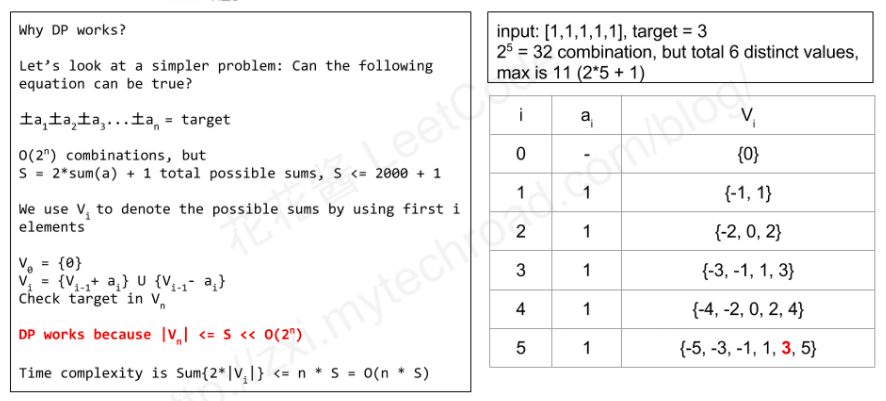
\includegraphics[width=.9\linewidth]{./pic/targetSum.png}

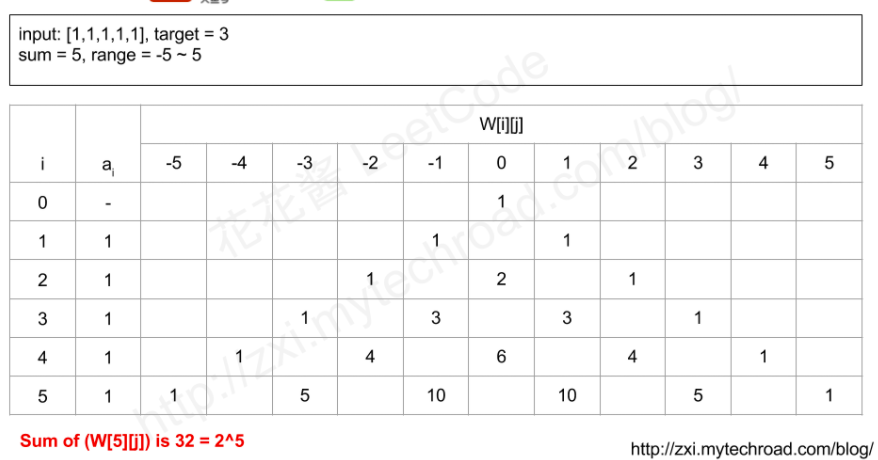
\includegraphics[width=.9\linewidth]{./pic/targetSum2.png}

\section{1477. Find Two Non-overlapping Sub-arrays Each With Target Sum}
\label{sec-1-52}
Given an array of integers arr and an integer target.
You have to find two non-overlapping sub-arrays of arr each with a sum equal target. There can be multiple answers so you have to find an answer where the sum of the lengths of the two sub-arrays is minimum.
Return the minimum sum of the lengths of the two required sub-arrays, or return -1 if you cannot find such two sub-arrays.
\begin{minted}[frame=lines,fontsize=\scriptsize,linenos=false]{java}
// 找出数组中等于target的最小非重叠区间的长度,用dp[i]表示当前i以及i之前的满足条件的最小区间长度,状态更新规则为
//     dp[i]=min(dp[i-1],i-j+1) if sum[j,i]=target
//     答案更新规则
//     res=min(res,dp[j−1]+i−j+1)
public int minSumOfLengths(int[] arr, int target) {
    int n = arr.length;
    int [] dp = new int [n];
    Arrays.fill(dp, Integer.MAX_VALUE);
    int cur = 0, s = 0;
    int res = Integer.MAX_VALUE, minLen = Integer.MAX_VALUE;
    for (int i = 0; i < n; i++) {
        cur += arr[i];
        while (cur > target) {
            cur -= arr[s];
            s += 1;
        }
        if (cur == target) {
            int curLen = i - s + 1;
            if (s > 0 && dp[s-1] != Integer.MAX_VALUE) 
                res = Math.min(res, curLen + dp[s-1]);
            minLen = Math.min(minLen, curLen);
        }
        dp[i] = minLen;
    }
    return res == Integer.MAX_VALUE ? -1 : res;
}
\end{minted}

\section{1771. Maximize Palindrome Length From Subsequences}
\label{sec-1-53}
You are given two strings, word1 and word2. You want to construct a string in the following manner:
Choose some non-empty subsequence subsequence1 from word1.
Choose some non-empty subsequence subsequence2 from word2.
Concatenate the subsequences: subsequence1 + subsequence2, to make the string.
Return the length of the longest palindrome that can be constructed in the described manner. If no palindromes can be constructed, return 0.
A subsequence of a string s is a string that can be made by deleting some (possibly none) characters from s without changing the order of the remaining characters.
A palindrome is a string that reads the same forward as well as backward.
\begin{minted}[frame=lines,fontsize=\scriptsize,linenos=false]{java}
public int longestPalindrome(String s, String t) { // 这个题目没有懂,需要再好好看一下
    int m = s.length();
    int n = t.length();
    int mn = m + n;
    String st = s + t;
    int [][] dp = new int [mn][mn];
    for (int i = 0; i < mn; i++)
        dp[i][i] = 1;
    for (int l = 2; l <= mn; l++) {
        for (int i = 0, j = i+l-1; j < mn; i++,j++) { // 
            if (st.charAt(i) == st.charAt(j))
                dp[i][j] = dp[i+1][j-1] + 2;
            else dp[i][j] = Math.max(dp[i+1][j], dp[i][j-1]);                         
        }
    }
    int ans = 0;
    for (int i = 0; i < m; i++) {
        for (int j = 0; j < n; j++) {
            if (s.charAt(i) == t.charAt(j))
                ans = Math.max(ans, dp[i][m+j]); // 
        }
    }
    return ans;
}
\end{minted}

\section{907. Sum of Subarray Minimums}
\label{sec-1-54}
Given an array of integers arr, find the sum of min(b), where b ranges over every (contiguous) subarray of arr. Since the answer may be large, return the answer modulo 109 + 7.
\begin{minted}[frame=lines,fontsize=\scriptsize,linenos=false]{java}
        public int sumSubarrayMins(int[] arr) {
            int n = arr.length;
            // for each A[i], find k <= i <= j, so that A[i] is the min from [k,j]
            // sum += A[i] * (i-k+1) * (j-i+1)
            // so we need to find the next min to the right and to the left
            //这个过程可以简化为使用一个栈。对于被某个数从栈中弹出的数而言,它右侧第一个比它小的数就是这个数。所以我们可以对所有被弹出的数得到左侧的区间范围和右侧的区间范围。我觉得这是一种非常聪明的做法。 这个栈我看得稀里糊涂,再想一下
            long [] right = new long [n];  // next smaller element index to the right 
            long [] left = new long[n];    // next smaller element index to the left
            Stack<Integer> s = new Stack<>();
            for (int i = 0; i < n; i++) {
                while (!s.isEmpty() && arr[i] <= arr[s.peek()]) {
                    right[s.pop()] = i-1;
                }
                s.push(i);
            }
            while (!s.isEmpty()) {
                right[s.pop()] = n-1;
            }
            s.clear();
            for (int i = n-1; i >= 0; i--) {
                while (!s.isEmpty() && arr[i] < arr[s.peek()])
                    left[s.pop()] = i+1;
                s.push(i);
            }
            while (!s.isEmpty())
                left[s.pop()] = 0;
            long sum = 0;
            long leftsize = 0, rightsize = 0;
            for (int i = 0; i < n; i++) {
                leftsize = i - left[i] +1;
                rightsize = right[i] - i + 1;
                sum += arr[i] * leftsize * rightsize;
                sum %= mod;
            }
            return (int)sum;
        }
        int mod = 1_000_000_007;
        public int sumSubarrayMins(int[] arr) {
            int n = arr.length;
            long [] left = new long[n];
            long [] right = new long[n];
            long sum = 0;
            long cnt = 0;
            int j = 0;
            for (int i = 0; i < n; i++) { // 计算左边比自身大的数的个数
                cnt = 1;
                j = i-1;
                while (j >= 0 && arr[j] >= arr[i]) {
                    cnt += left[j];
                    j -= left[j];
                }
                left[i] = cnt;
            }
            // 就是因为计算了两个方向,所以对于数组里面有相同元素的情况下,需要特别考虑一下。
            //     不能重复计算, 也不能漏掉,
            //     具体就是一个方向的时候用<=, 另外一个方向的时候用<。 这个在做的时候也bug了。
            for (int i = n-1; i >= 0; i--) { // 计算右边比自身大的数的个数
                cnt = 1;
                j = i+1;
                while (j < n && arr[j] > arr[i]) {
                    cnt += right[j];
                    j += right[j];
                }
                right [i] = cnt;
            }
            for (int i = 0; i < n; i++) 
                sum += arr[i] * left[i] * right[i];
            return (int) (sum % mod);
        }
\end{minted}

\section{689. Maximum Sum of 3 Non-Overlapping Subarrays}
\label{sec-1-55}
Given an integer array nums and an integer k, find three non-overlapping subarrays of length k with maximum sum and return them.
Return the result as a list of indices representing the starting position of each interval (0-indexed). If there are multiple answers, return the lexicographically smallest one.
\begin{minted}[frame=lines,fontsize=\scriptsize,linenos=false]{java}
public int[] maxSumOfThreeSubarrays(int[] nums, int k) {
    int n = nums.length;
    int [] pre = new int [n+1];
    for (int i = 1; i <= n; i++) 
        pre[i] = pre[i-1] + nums[i-1];
    // left[i]表示在区间[0, i]范围内长度为k且和最大的子数组的起始位置
    // right[i]表示在区间[i, n - 1]范围内长度为k且和最大的子数组的起始位置
    int [] left = new int [n];
    int [] right = new int [n];
    int [] res = new int [3];
    Arrays.fill(right, n-k);
    for (int i = k, total = pre[k]-pre[0]; i < n; i++) {
        if (pre[i+1] - pre[i+1-k] > total) {
            left[i]= i+1-k;
            total = pre[i+1] - pre[i+1-k];
        } else left[i] = left[i-1];
    }
    for (int i = n-1-k, total = pre[n]-pre[n-k]; i >= 0; i--) {
        if (pre[i+k] - pre[i] >= total) {
            right[i] = i;
            total = pre[i+k] - pre[i];
        } else right[i] = right[i+1];
    }
    int max = Integer.MIN_VALUE;
    for (int i = k; i <= n-2*k; i++) {
        int l = left[i-1];
        int r = right[i+k];
        int total = (pre[i+k]-pre[i]) + (pre[k+l]-pre[l]) + (pre[r+k] - pre[r]);
        if (max < total) {
            max = total;
            res = new int [] {l, i, r};
        }
    }
    return res;
}
\end{minted}

\section{363. Max Sum of Rectangle No Larger Than K}
\label{sec-1-56}
Given an m x n matrix matrix and an integer k, return the max sum of a rectangle in the matrix such that its sum is no larger than k.
It is guaranteed that there will be a rectangle with a sum no larger than k.
\begin{minted}[frame=lines,fontsize=\scriptsize,linenos=false]{java}
public int maxSumSubmatrix(int[][] mat, int k) {
    int m = mat.length;
    int n = mat[0].length;
    if (m == 1 && n == 1) return mat[0][0];
    int [][] pre = new int [m][n];
    int res = Integer.MIN_VALUE;
    for (int i = 0; i < m; i++) {
        for (int j = 0; j < n; j++) {
            int t = mat[i][j];
            if (i > 0) t += pre[i-1][j];
            if (j > 0) t += pre[i][j-1];
            if (i > 0 && j > 0) t -= pre[i-1][j-1];
            pre[i][j] = t;
            for (int r = 0; r <= i; r++) {
                for (int c = 0; c <= j; c++) {
                    int d = pre[i][j];
                    if (r > 0) d -= pre[r-1][j];
                    if (c > 0) d -= pre[i][c-1];
                    if (r > 0 && c > 0) d += pre[r-1][c-1];
                    if (d <= k) res = Math.max(res, d);
                }
            }
        }
    }
    return res;
}
// 把二维数组按行或列拆成多个一维数组,然后利用一维数组的累加和来找符合要求的数字,
// 这里用了 lower_bound 来加快的搜索速度,也可以使用二分搜索法来替代。
public int maxSumSubmatrix(int[][] mat, int target) {
    int row = mat.length;
    int col = mat[0].length;
    int res = Integer.MIN_VALUE;
    boolean key = col > row ? false : true;
    int m = Math.min(row, col);
    int n = Math.max(row, col);
    int [] pre = new int [n];
    TreeSet<Integer> ts = new TreeSet<>(); //用来保存当前高度下,长度为从0开始到k位置的矩形的结果。理解set的含义是解决此题的关键。
    Integer tmp = 0;
    for (int i = 0; i < m; i++) { // 找从第i行开始一直到第0行这i+1行的可能组成的矩形长度
        Arrays.fill(pre, 0);
        for (int j = i; j >= 0; j--) {
            ts.clear();
            ts.add(0);
            int curSum = 0;
            for (int k = 0; k < n; k++) {
                if (key)
                    pre[k] += mat[k][j];
                else pre[k] += mat[j][k];
                curSum += pre[k];
                 // * 因为要满足  (sum-set中的元素)<=target,
                 // * 而且sum-set中的元素的值要尽可能的大,
                 // * 所以也就是再求小于等于sum-target中满足条件的元素的最小的一个
                 // * 正好TreeSet中提供了这个方法ceil(),可以很方便的找出这个元素
                tmp = ts.ceiling(curSum - target);
                if (tmp != null) res = Math.max(res, curSum - tmp);
                ts.add(curSum);
            }
        }
    }
    return res;
}
\end{minted}

\section{805. Split Array With Same Average}
\label{sec-1-57}
You are given an integer array nums.
You should move each element of nums into one of the two arrays A and B such that A and B are non-empty, and average(A) == average(B).
Return true if it is possible to achieve that and false otherwise.
Note that for an array arr, average(arr) is the sum of all the elements of arr over the length of arr.
\begin{minted}[frame=lines,fontsize=\scriptsize,linenos=false]{java}
public boolean splitArraySameAverage(int[] nums) {
    int n = nums.length;
    int m = n / 2;
    int sum = Arrays.stream(nums).sum();
    boolean poss = false;
    for (int i = 1; i <= m; i++) 
        if (sum * i % n == 0) {
            poss = true;
            break;
        }
    if (!poss) return false;
    List<Set<Integer>> ls = new ArrayList<>();
    for (int i = 0; i <= m; i++) 
        ls.add(new HashSet<Integer>());
    ls.get(0).add(0);    // 这种构建子序列和的方法,要学习一下
    for (int v : nums)  // for each element in A, we try to add it to sums[i] by joining sums[i - 1]
        for (int i = m; i >= 1; i--) 
            for (int t : ls.get(i-1)) 
                ls.get(i).add(t + v);
    for (int i = 1; i <= m; i++) {
        if (sum * i % n == 0 && ls.get(i).contains(sum * i / n))
            return true;
    }
    return false;
}
\end{minted}

\section{1981. Minimize the Difference Between Target and Chosen Elements}
\label{sec-1-58}
You are given an m x n integer matrix mat and an integer target.
Choose one integer from each row in the matrix such that the absolute difference between target and the sum of the chosen elements is minimized.
Return the minimum absolute difference.
The absolute difference between two numbers a and b is the absolute value of a - b.
\begin{minted}[frame=lines,fontsize=\scriptsize,linenos=false]{java}
// DP + BitSet : 这里面有个小问题需要挑出来
// 使用一个DP数组存下当前行和之前行每行选一个数可能构成的和,
// 在本题中,可以使用BitSet(简介)来存储之前行可以组成的和(由于所有数的最大值为70,而行数最大也为70,故BitSet最大的位数即为4900)。
// 对于当前行,遍历BitSet已经set过的位(即代表之前行可能组成的和),然后加上当前数,set新的和
// 最后遍历BitSet,求出当前位与target的最小值
public int minimizeTheDifference(int[][] mat, int target) {
    int m = mat.length;
    int n = mat[0].length;
    BitSet sum = new BitSet(); // 遍历每一行,存下当前行和之前行可能组成的和
    for (int i = 0; i < n; i++) // 初始时存下第一行
        sum.set(mat[0][i]);
    for (int i = 1; i < m; i++) {
        BitSet newSum = new BitSet(); // 用来存新的和
        for (int j = 0; j < n; j++) {
            // 注意:要遍历BitSet中的真实位,请使用以下循环:previousSetBit()方法 用于查找在指定的起始索引上或之前是否存在任何真位
            // for (int i = bs.length(); (i = bs.previousSetBit(i-1)) >= 0; ) {
            //     // operate on index i here
            // }
            for (int k = sum.length(); (k = sum.previousSetBit(k-1)) >= 0; ) {
                newSum.set(k+mat[i][j]);
            }
        }
        sum = newSum;
    }
    int ans = 4900;
    for (int k = sum.length(); (k = sum.previousSetBit(k-1)) >= 0;) {
        int diff = Math.abs(k - target);
        ans = Math.min(ans, diff);
    }
    return ans;
}
public int minimizeTheDifference(int[][] mat, int target) {
    int m = mat.length;
    int n = mat[0].length;
    int diff = Integer.MAX_VALUE, limit = 4900;
    int [] dp = new int[limit];
    for (int i = 0; i < n; i++) // 相当于是手工实现java BitSet
        dp[mat[0][i]] = 1;
    for (int i = 1; i < m; i++) {
        int [] tmp = new int [limit];
        for (int v = limit-1; v >= 0; v--) {
            if (dp[v] == 0) continue;
            for (int j = 0; j < n; j++) {
                if (v + mat[i][j] < limit)
                    tmp[v+mat[i][j]] = 1;
            }
        }
        System.arraycopy(tmp, 0, dp, 0, dp.length);
    }
    for (int i = 0; i < limit; i++) 
        if (dp[i] > 0) diff = Math.min(diff, Math.abs(i-target));
    return diff;  // min difference
}
\end{minted}

\section{805. Split Array With Same Average}
\label{sec-1-59}
You are given an integer array nums.
You should move each element of nums into one of the two arrays A and B such that A and B are non-empty, and average(A) == average(B).
Return true if it is possible to achieve that and false otherwise.
Note that for an array arr, average(arr) is the sum of all the elements of arr over the length of arr.
\begin{minted}[frame=lines,fontsize=\scriptsize,linenos=false]{java}
    //     1)如果一个长度为n的数组可以被划分为A和B两个数组,我们假设A的长度小于B并且A的大小是k,那么:total_sum / n == A_sum / k == B_sum / (n - k),其中1 <= k <= n / 2。那么可以知道:A_sum = total_sum * k / n。由于A_sum一定是个整数,所以我们可以推导出total_sum * k % n == 0,那就是说,对于特定的total_sum和n而言,符合条件的k不会太多。这样我们在第一步中就首先验证是否存在符合条件的k,如果不存在就可以提前返回false。
    //     2)如果经过第一步的验证,发现确实有符合条件的k,那么我们在第二步中,就试图产生k个子元素的所有组合,并且计算他们的和。这里的思路就有点类似于背包问题了,vector<unordered_set<int>> sums,其中sums[i][j]表示A[0, i]这个子数组中的任意j个元素的所有可能和。可以得到递推公式是:sums[i][j] = sums[i - 1][j] "join" (sums[i][j - 1] + A[i]),其中等式右边的第一项表示这j个元素中不包含A[i],而第二项表示这j个元素包含A[i]。这样就可以采用动态规划的思路得到sums[n - 1][k]了(1 <= k <= n / 2)。
    // 3)有了sums[n - 1][k],我们就检查sums[n - 1][k]中是否包含(total_sum * k / n)。一旦发现符合条件的k,就返回true,否则就返回false。
    // 在递推公式中我们发现,sums[i][j]仅仅和sums[i - 1][j],sums[i][j - 1]有关,所以可以进一步将空间复杂度从O(n^2*M)降低到O(n*M),其中M是n中的所有元素的组合数(可能高达O(2^n))。时间复杂度为O(n^3*M)。
public boolean splitArraySameAverage(int[] nums) {
    int n = nums.length;
    int m = n / 2;
    int sum = Arrays.stream(nums).sum();
    boolean poss = false;
    for (int i = 1; i <= m; i++) {
        if (sum * i % n == 0) {
            poss = true;
            break;
        }
    }
    if (!poss) return false;
    List<Set<Integer>> ls = new ArrayList<>();
    for (int i = 0; i <= m; i++) 
        ls.add(new HashSet<Integer>());
    ls.get(0).add(0);    // 这种构建子序列和的方法,要学习一下
    for (int v : nums) { // for each element in A, we try to add it to sums[i] by joining sums[i - 1]
        for (int i = m; i >= 1; i--) {
            for (int t : ls.get(i-1)) {
                ls.get(i).add(t + v);
            }
        }
    }
    // System.out.println("ls.size(): " + ls.size());
    // for (int z = 0; z < ls.size(); ++z) {
    //     for (Integer x : ls.get(z))
    //         System.out.print(x + ", ");
    //     System.out.print("\n");
    //     System.out.print("\n ");
    // }
    for (int i = 1; i <= m; i++) {
        if (sum * i % n == 0 && ls.get(i).contains(sum * i / n))
            return true;
    }
    return false;
}
private boolean helper(int [] arr, int curSum, int cur, int start) {
    if (cur == 0) return curSum == 0;
    if (arr[start] > curSum / cur) return false;
    for (int i = start; i < arr.length - cur + 1; i++) {
        if (i > start && arr[i] == arr[i-1]) continue;
        if (helper(arr, curSum - arr[i], cur-1, i+1)) return true;
    }
    return false;
}
public boolean splitArraySameAverage(int[] nums) {
    int n = nums.length;
    int m = n / 2;
    int sum = Arrays.stream(nums).sum();
    boolean poss = false;
    for (int i = 1; i <= m; i++) {
        if (sum * i % n == 0) {
            poss = true;
            break;
        }
    }
    if (!poss) return false;
    Arrays.sort(nums);
    for (int i = 1; i <= m; i++) 
        if (sum * i % n == 0 && helper(nums, sum * i / n, i, 0)) return true;
    return false;
}
bool splitArraySameAverage(vector<int>& A) {  // https://www.cnblogs.com/grandyang/p/10285531.html
    int n = A.size(), m = n / 2, sum = accumulate(A.begin(), A.end(), 0);
    bool possible = false;
    for (int i = 1; i <= m && !possible; ++i) {
        if (sum * i % n == 0) possible = true;
    }
    if (!possible) return false;
    bitset<300001> bits[m + 1] = {1};
    for (int num : A) {
        for (int i = m; i >= 1; --i) {
            bits[i] |= bits[i - 1] << num;
        }
    }
    for (int i = 1; i <= m; ++i) {
        if (sum * i % n == 0 && bits[i][sum * i / n]) return true;
    }
    return false;
}
\end{minted}

\section{801. Minimum Swaps To Make Sequences Increasing - Hard}
\label{sec-1-60}
You are given two integer arrays of the same length nums1 and nums2. In one operation, you are allowed to swap nums1[i] with nums2[i].

For example, if nums1 = [1,2,3,8], and nums2 = [5,6,7,4], you can swap the element at i = 3 to obtain nums1 = [1,2,3,4] and nums2 = [5,6,7,8].
Return the minimum number of needed operations to make nums1 and nums2 strictly increasing. The test cases are generated so that the given input always makes it possible.

An array arr is strictly increasing if and only if arr\footnotemark[2]{} < arr\footnotemark[3]{} < arr\footnotemark[5]{} < \ldots{} < arr[arr.length - 1].
\begin{minted}[frame=lines,fontsize=\scriptsize,linenos=false]{java}
// 设 dp[0][i] 表示不交换 A[i] 和 B[i] 在下标 i 的交换次数
// 设 dp[1][i] 表示交换 A[i] 和 B[i] 在下标 i 的交换次数
// 可以看到交换与否只取决与前一个状态, 可以将空间复杂度压缩到 O(1)
//     时间复杂度为 O(n), 空间复杂度为 O(1)
public int minSwap(int[] a, int[] b) {
    int n = a.length;
    int [][] dp = new int [2][n];
    for (int [] row : dp) 
        Arrays.fill(row, Integer.MAX_VALUE);
    dp[0][0] = 0;
    dp[1][0] = 1;
    for (int i = 1; i < n; i++) {
        if (a[i] > a[i-1] && b[i] > b[i-1]) {
            dp[0][i] = Math.min(dp[0][i], dp[0][i-1]);    // 不需要交换不用增加交换次数
            dp[1][i] = Math.min(dp[1][i], dp[1][i-1] + 1);// 如果要交换前一个也必须交换才能满足递增的条件
        }
        if (a[i] > b[i-1] && b[i] > a[i-1]) {
            dp[0][i] = Math.min(dp[0][i], dp[1][i-1]);    // 表示 i - 1 位置发生交换  
            dp[1][i] = Math.min(dp[1][i], dp[0][i-1] + 1);// 表示在 i - 1 不换的基础上, i 发生了交换 
        }
    }
    return Math.min(dp[0][n-1], dp[1][n-1]);
}
\end{minted}
\section{837. New 21 Game - Medium}
\label{sec-1-61}
Alice plays the following game, loosely based on the card game "21".

Alice starts with 0 points and draws numbers while she has less than k points. During each draw, she gains an integer number of points randomly from the range [1, maxPts], where maxPts is an integer. Each draw is independent and the outcomes have equal probabilities.

Alice stops drawing numbers when she gets k or more points.

Return the probability that Alice has n or fewer points.

Answers within 10-5 of the actual answer are considered accepted.
\begin{minted}[frame=lines,fontsize=\scriptsize,linenos=false]{java}
// When the draws sum up to K, it stops, calculate the possibility K<=sum<=N.
//     Think about one step earlier, sum = K-1, game is not ended and draw largest card W.
//     K-1+W is the maximum sum could get when game is ended. If it is <= N, then for sure the possiblity when games end ans sum <= N is 1.
//     Because the maximum is still <= 1.
//     Otherwise calculate the possibility sum between K and N.
//     Let dp[i] denotes the possibility of that when game ends sum up to i.
//     i is a number could be got equally from i - m and draws value m card.
//     Then dp[i] should be sum of dp[i-W] + dp[i-W+1] + ... + dp[i-1], devided by W.
//     We only need to care about previous W value sum, accumlate winSum, reduce the possibility out of range.
//     Time Complexity: O(N).
//     Space: O(N).
public double new21Game(int n, int k, int w) { // k : threshold
    if (k == 0 || n >= (k + w)) return 1.0;
    if (k > n) return 0;
    double [] dp = new double [n+1];
    dp[0] = 1.0;
    double winSum = 1;
    double res = 0;
    for (int i = 1; i <= n; i++) {
        dp[i] = winSum / w;
        if (i < k) winSum += dp[i];
        else res += dp[i];
        if (i >= w) winSum -= dp[i-w];
    }
    return res;
}
\end{minted}
\section{1105. Filling Bookcase Shelves - Medium}
\label{sec-1-62}
You are given an array books where books[i] = [thicknessi, heighti] indicates the thickness and height of the ith book. You are also given an integer shelfWidth.

We want to place these books in order onto bookcase shelves that have a total width shelfWidth.

We choose some of the books to place on this shelf such that the sum of their thickness is less than or equal to shelfWidth, then build another level of the shelf of the bookcase so that the total height of the bookcase has increased by the maximum height of the books we just put down. We repeat this process until there are no more books to place.

Note that at each step of the above process, the order of the books we place is the same order as the given sequence of books.

For example, if we have an ordered list of 5 books, we might place the first and second book onto the first shelf, the third book on the second shelf, and the fourth and fifth book on the last shelf.
Return the minimum possible height that the total bookshelf can be after placing shelves in this manner.
\begin{minted}[frame=lines,fontsize=\scriptsize,linenos=false]{java}
// 求摆放前i本书需要的最小高度,首先需要求摆放前i-1书需要的最小高度,以此类推,最初需要计算的是摆放第0本书需要的最小高度,也就是0。
// 根据前i-1本书求前i书需要的最小高度的思路是:
// 尝试①将第i本书放在前i-1本书的下面
// 以及②将前i-1本书的最后几本和第i本书放在同一层两种方案,看哪种方案高度更小就用哪种方案,依次求出摆放前1,…,n本书需要的最小高度。
public int minHeightShelves(int[][] books, int shelfWidth) {
    int [] dp = new int [books.length + 1];
    for (int i = 1; i < dp.length; i++) { // 依次求摆放前i本书的最小高度
        int width = books[i-1][0];
        int height = books[i-1][1];
        dp[i] = dp[i-1] + height;
        // 将前i - 1本书从第i - 1本开始放在与i同一层,直到这一层摆满或者所有的书都摆好
        for (int j = i-1; j > 0 && width + books[j-1][0] <= shelfWidth; j--) {
            height = Math.max(height, books[j-1][1]); // 每层的高度由最高的那本书决定
            width += books[j-1][0];
            dp[i] = Math.min(dp[i], dp[j-1] + height);// 选择高度最小的方法
        }
    }            
    return dp[books.length];
}
\end{minted}
\section{1997. First Day Where You Have Been in All the Rooms - Medium}
\label{sec-1-63}
There are n rooms you need to visit, labeled from 0 to n - 1. Each day is labeled, starting from 0. You will go in and visit one room a day.

Initially on day 0, you visit room 0. The order you visit the rooms for the coming days is determined by the following rules and a given 0-indexed array nextVisit of length n:

Assuming that on a day, you visit room i,
if you have been in room i an odd number of times (including the current visit), on the next day you will visit a room with a lower or equal room number specified by nextVisit[i] where 0 <= nextVisit[i] <= i;
if you have been in room i an even number of times (including the current visit), on the next day you will visit room (i + 1) mod n.
Return the label of the first day where you have been in all the rooms. It can be shown that such a day exists. Since the answer may be very large, return it modulo 109 + 7.
\begin{minted}[frame=lines,fontsize=\scriptsize,linenos=false]{java}
public int firstDayBeenInAllRooms(int [] nextVisit) {
    int n = nextVisit.length, mod = (int)1e9 + 7;
    long [] dp = new long [n];
    dp[0] = 0;
    for (int i = 1; i < n; i++) 
        dp[i] = (2 * dp[i-1] % mod + mod - dp[nextVisit[i-1]] + 2) % mod;
    return (int)dp[n-1];
}
\end{minted}

\section{943. Find the Shortest Superstring - Hard}
\label{sec-1-64}
Given an array of strings words, return the smallest string that contains each string in words as a substring. If there are multiple valid strings of the smallest length, return any of them.

You may assume that no string in words is a substring of another string in words.
\begin{itemize}
\item 深搜 + 记忆数组 + 裁枝
\end{itemize}
\begin{minted}[frame=lines,fontsize=\scriptsize,linenos=false]{java}
private void dfs(int [] tmp, int idx, int curCost, boolean [] vis, int path) {
    if (idx == n) {
        if (curCost > maxCost) {
            maxCost = curCost;
            best = Arrays.copyOf(tmp, n); // best = tmp.clone();
        }
        return;
    }
    for (int i = 0; i < n; i++) 
        if (!vis[i]) {
            int tmpCost = idx == 0 ? 0 : curCost + cost[tmp[idx-1]][i];
            int tmpPath = (path | (1 << i));
            int maxCost = dp[tmpPath][i];
            if (maxCost > 0 && tmpCost <= maxCost) continue;
            tmp[idx] = i;
            dp[tmpPath][i] = tmpCost; // need to remember the res
            vis[i] = true;
            dfs(tmp, idx+1, tmpCost, vis, tmpPath);
            vis[i] = false;
        }
}
int n, maxCost = Integer.MIN_VALUE; // 最长公共子串的长度和,越大越好
int [][] dp;
int [][] cost;
int [] best;
public String shortestSuperstring(String[] words) {
    n = words.length;
    cost = new int [n][n];
    for (int i = 0; i < n; i++) 
        for (int j = 0; j < n; j++) {
            if (i == j) continue;
            for (int k = 1; k <= words[i].length() && k <= words[j].length(); k++) {
                if (words[i].substring(words[i].length()-k).equals(words[j].substring(0, k)))
                    cost[i][j] = k;
            }
        }
    dp = new int [1 << n][n];
    best = new int [n];
    dfs(new int [n], 0, 0, new boolean [n], 0);
    String res = words[best[0]];
    for (int i = 1; i < n; i++) {
        int costVal = cost[best[i-1]][best[i]];
        res += words[best[i]].substring(costVal);
    }
    return res;
}
\end{minted}
\begin{itemize}
\item 动态规划
\end{itemize}
\begin{minted}[frame=lines,fontsize=\scriptsize,linenos=false]{java}
public String shortestSuperstring(String[] words) {
    int n = words.length;
    String [][] dp = new String [1 << n][n];
    int [][] overlap = new int [n][n];
    for (int i = 0; i < n; i++) 
        for (int j = 0; j < n; j++) {
            if (i == j) continue;
            for (int k = Math.min(words[i].length(), words[j].length()); k > 0; k--) {
                if (words[i].substring(words[i].length()-k).equals(words[j].substring(0, k))) {
                    overlap[i][j] = k;
                    break;
                }
            }
        }
    for (int i = 0; i < n; i++)
        dp[1 << i][i] = words[i];
    for (int mask = 1; mask < (1 << n); mask++) 
        for (int j = 0; j < n; j++) {
            if ((mask & (1 << j)) == 0) continue;
            for (int i = 0; i < n; i++) {
                if (i == j || (mask & (1 << i)) == 0) continue;
                String tmp = dp[mask ^ (1 << j)][i] + words[j].substring(overlap[i][j]);
                if (dp[mask][j] == null || tmp.length() < dp[mask][j].length()) // str.isEmpty()
                    dp[mask][j] = tmp;
            }
        }
    int last = (1 << n) - 1;
    String res = dp[last][0];
    for (int i = 1; i < n; i++) 
        if (dp[last][i].length() < res.length())
            res = dp[last][i];
    return res;
}
\end{minted}

\section{964. Least Operators to Express Number - Hard}
\label{sec-1-65}
Given a single positive integer x, we will write an expression of the form x (op1) x (op2) x (op3) x \ldots{} where each operator op1, op2, etc. is either addition, subtraction, multiplication, or division (+, -, *, or /). For example, with x = 3, we might write 3 * 3 / 3 + 3 - 3 which is a value of 3.

When writing such an expression, we adhere to the following conventions:

The division operator (/) returns rational numbers.
There are no parentheses placed anywhere.
We use the usual order of operations: multiplication and division happen before addition and subtraction.
It is not allowed to use the unary negation operator (-). For example, "x - x" is a valid expression as it only uses subtraction, but "-x + x" is not because it uses negation.
We would like to write an expression with the least number of operators such that the expression equals the given target. Return the least number of operators used.

博主看了一会儿,发现没思路就直接放弃了,直奔论坛上找解法。这里直接参考 donggua$_{\text{fu}}$ 大神的解法吧,首先处理 edge cases,当 x 等于 target 的话,不用加任何运算符,返回0即可。若 x 大于 target,比如 x=5,target=3,我们其实可以迅速的求出运算符的个数,因为5比3大,要凑3就只能先变成1,这里就有两种变法,一种是全部都变成1,然后来凑3,即 5/5 + 5/5 + 5/5,这时的运算符个数是 target * 2 -1,因为加号的个数总是比除号少一个。另一种凑法就是 5 - 5/5 - 5/5,这时候的运算符个数是 (x - target) * 2,此时的加号和除号的个数相同,均为x和 target 的差值。

接下来就要处理 x 小于 target 的情况了,此时由于不知道x到底比 target 小多少,若差距太大的话,肯定不能用加号,所以应该先用乘号来让x变大,直到刚好大于等于 target 停止,并每次增加次数 cnt。若此时 sum 正好等于 target,太幸运了,直接返回 cnt。但通常情况下 sum 会大于 target,此时 sum - target 的差值就需要另行计算了。这里差值跟 target 的大小关系又要分为两种情况来讨论,当 sum - target < target 时,比如 x=5,sum=25,target=15,则 sum - target=10,就是说现在已经乘到了 25,但需要再减去 10,这个差值 10 可以再次调用原函数来计算,此时新的 target 代入 10 即可,记得返回值要加上 cnt。当然之后还是要再计算一下另一种凑的方法,由于 sum 超过了 target,所以回退一个x,变成 sum / x,此时小于 target,那么它们的差值 target - (sum / x) 就可以通过再次调用函数来计算,注意这里加上 cnt 之后还要减去1,因为回退了一个x,少了一个乘号。最终二者的较小值即为所求,记得要加上个1,以为多加了个运算符,参见代码如下:

\begin{minted}[frame=lines,fontsize=\scriptsize,linenos=false]{java}
public int leastOpsExpressTarget(int x, int target) {
    if (x == target) return 0;
    if (x > target) return Math.min(target*2-1, (x-target)*2);
    int cnt = 0;
    long sum = x;
    while (sum  < target) {
        sum *= x;
        ++cnt;
    }
    if (sum == target) return cnt;
    int min = Integer.MAX_VALUE, max = Integer.MIN_VALUE;
    // int tmp = sum - target; // -
    if (sum - target < target)
        min = leastOpsExpressTarget(x, (int)(sum - target)) + cnt;
    max = leastOpsExpressTarget(x, (int)(target - (sum / x))) + cnt - 1;
    return Math.min(min, max) + 1; // -
}
\end{minted}
\begin{itemize}
\item 和race car 那道题类似。注意到,符号的添加就是对数字 进行 -x$^{\text{i}}$ 的操作,最后要减到0,k = logx(t),有两种方式,可以先到 t 前面的数字,2$^{\text{k}}$, 或者 t后面的数字 2$^{\text{(k+1)}}$。
\end{itemize}
注意,2$^{\text{k需要的符号是k,最后因为第一个一定可以是正的,省一个符号。}}$

看了花花酱的题解,感觉更像是bfs。cost小的点先扩展。 \textbf{这个再看一下}

\begin{minted}[frame=lines,fontsize=\scriptsize,linenos=false]{cpp}
int leastOpsExpressTarget(int x, int target) {
    priority_queue<pair<int, int>, vector<pair<int, int>>, greater<pair<int, int>>> que;
    unordered_set<int> s;
    que.emplace(0, target);
    while(!que.empty()) {
        int cost = que.top().first;
        int t = que.top().second;
        que.pop();
        if (t == 0) return cost-1;
        if (s.count(t)) continue;
        s.insert(t);
        int k = log(t) / log(x);
        int l = t - pow(x, k);
        que.emplace(cost+(k == 0 ? 2 : k), l);
        int r = pow(x, k+1) - t;
        que.emplace(cost+k+1, r);
    }
    return -1;
}
\end{minted}
\section{1955. Count Number of Special Subsequences - Hard}
\label{sec-1-66}
A sequence is special if it consists of a positive number of 0s, followed by a positive number of 1s, then a positive number of 2s.

For example, [0,1,2] and [0,0,1,1,1,2] are special.
In contrast, [2,1,0], \footnotemark[3]{}, and [0,1,2,0] are not special.
Given an array nums (consisting of only integers 0, 1, and 2), return the number of different subsequences that are special. Since the answer may be very large, return it modulo 109 + 7.

A subsequence of an array is a sequence that can be derived from the array by deleting some or no elements without changing the order of the remaining elements. Two subsequences are different if the set of indices chosen are different.

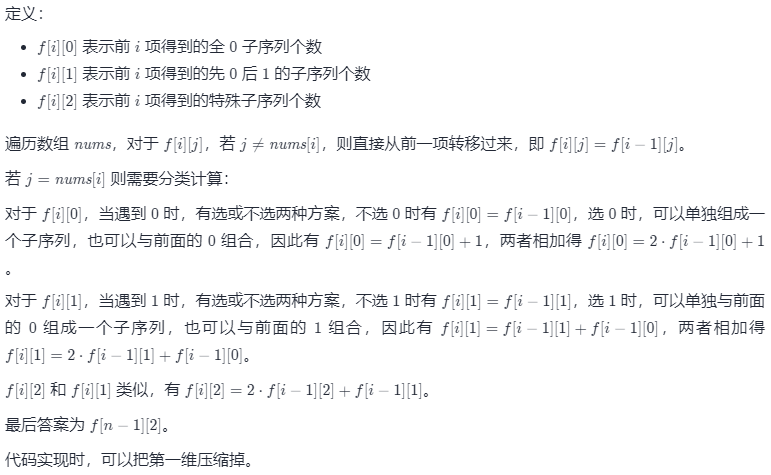
\includegraphics[width=.9\linewidth]{./pic/specialSeq.png}

\begin{minted}[frame=lines,fontsize=\scriptsize,linenos=false]{java}
public int countSpecialSubsequences(int[] arr) { // 去找个降维的参考一下
    int mod = (int)1e9 + 7;
    int n = arr.length;
    long [][] dp = new long [n][3];
    for (int i = 0; i < n; i++) 
        for (int j = 0; j < 3; j++) {
            if (arr[i] != j) dp[i][j] = (i == 0 ? 0 : dp[i-1][j]);
            else 
                if (j == 0)
                    dp[i][j] = (i == 0 ? 0 : dp[i-1][j]) * 2 % mod + 1;
                else
                    dp[i][j] = ((i == 0 ? 0 : dp[i-1][j]) * 2 % mod + (i == 0 ? 0 : dp[i-1][j-1])) % mod;
        }
    return (int)dp[n-1][2];
}
\end{minted}

\section{446. Arithmetic Slices II - Subsequence - Hard}
\label{sec-1-67}
Given an integer array nums, return the number of all the arithmetic subsequences of nums.

A sequence of numbers is called arithmetic if it consists of at least three elements and if the difference between any two consecutive elements is the same.

For example, [1, 3, 5, 7, 9], [7, 7, 7, 7], and [3, -1, -5, -9] are arithmetic sequences.
For example, [1, 1, 2, 5, 7] is not an arithmetic sequence.
A subsequence of an array is a sequence that can be formed by removing some elements (possibly none) of the array.

For example, [2,5,10] is a subsequence of [1,2,1,2,4,1,5,10].
The test cases are generated so that the answer fits in 32-bit integer.
\subsection{解题思路与分析}
\label{sec-1-67-1}
这道题是之前那道Arithmetic Slices的延伸,那道题比较简单是因为要求等差数列是连续的,而这道题让我们求是等差数列的子序列,可以跳过某些数字,不一定非得连续,那么难度就加大了,但还是需要用动态规划Dynamic Progrmming来做。

好,既然决定要用DP了,那么首先就要确定dp数组的定义了,刚开始我们可能会考虑使用个一维的dp数组,然后dp[i]定义为范围为[0, i]的子数组中等差数列的个数。定义的很简单,OK,但是基于这种定义的状态转移方程却十分的难想。我们想对于(0, i)之间的任意位置j,如何让 dp[i] 和 dp[j] 产生关联呢?是不是只有 A[i] 和 A[j] 的差值diff,跟A[j]之前等差数列的差值相同,才会有关联,所以差值diff是一个很重要的隐藏信息Hidden Information,我们必须要在dp的定义中考虑进去。所以一维dp数组是罩不住的,必须升维,但是用二维dp数组的话,差值diff那一维的范围又是个问题,数字的范围是整型数,所以差值的范围也很大,为了节省空间,我们建立一个一维数组dp,数组里的元素不是数字,而是放一个HashMap,建立等差数列的差值和当前位置之前差值相同的数字个数之间的映射。我们遍历数组中的所有数字,对于当前遍历到的数字,又从开头遍历到当前数字,计算两个数字之差diff,如果越界了不做任何处理,如果没越界,我们让dp[i]中diff的差值映射自增1,因为此时A[i]前面有相差为diff的A[j],所以映射值要加1。然后我们看dp[j]中是否有diff的映射,如果有的话,说明此时相差为diff的数字至少有三个了,已经能构成题目要求的等差数列了,将dp[j][diff]加入结果res中,然后再更新dp[i][diff],这样等遍历完数组,res即为所求。

我们用题目中给的例子数组 [2,4,6,8,10] 来看,因为2之前没有数字了,所以我们从4开始,遍历前面的数字,是2,二者差值为2,那么在dp\footnotemark[3]{}的HashMap就可以建立 2->1 的映射,表示4之前有1个差值为2的数字,即数字2。那么现在i=2指向6了,遍历前面的数字,第一个数是2,二者相差4,那么在dp\footnotemark[5]{}的HashMap就可以建立 4->1 的映射,第二个数是4,二者相差2,那么先在dp\footnotemark[5]{}的HashMap建立 2->1 的映射,由于dp\footnotemark[3]{}的HashMap中也有差值为2的映射,2->1,那么说明此时至少有三个数字差值相同,即这里的 [2 4 6],我们将dp\footnotemark[3]{}中的映射值加入结果res中,然后当前dp\footnotemark[5]{}中的映射值加上dp\footnotemark[3]{}中的映射值。这应该不难理解,比如当i=3指向数字8时,j=2指向数字6,那么二者差值为2,此时先在dp\footnotemark[1]{}建立 2->1 的映射,由于dp\footnotemark[5]{}中有 2->2 的映射,那么加上数字8其实新增了两个等差数列 [2,4,6,8] 和 [4,6,8],所以结果res加上的值就是 dp[j][diff],即2,并且 dp[i][diff] 也需要加上这个值,才能使得 dp\footnotemark[1]{} 中的映射变为 2->3 ,后面数字10的处理情况也相同,这里就不多赘述了,最终的各个位置的映射关系如下所示:
\begin{minted}[frame=lines,fontsize=\scriptsize,linenos=false]{java}
2     4     6     8     10    
     2->1  4->1  6->1  8->1
           2->2  4->1  6->1 
                 2->3  4->2
                       2->4
\end{minted}

最终累计出来的结果是跟上面红色的数字相关,分别对应着如下的等差数列:

\begin{minted}[frame=lines,fontsize=\scriptsize,linenos=false]{java}
2->2:[2,4,6]
2->3:[2,4,6,8]    [4,6,8]
4->2:[2,6,10]
2->4:[2,4,6,8,10]    [4,6,8,10]    [6,8,10]
\end{minted}
\begin{itemize}
\item Both time and space complexities are O(n$^{\text{2}}$)
\end{itemize}

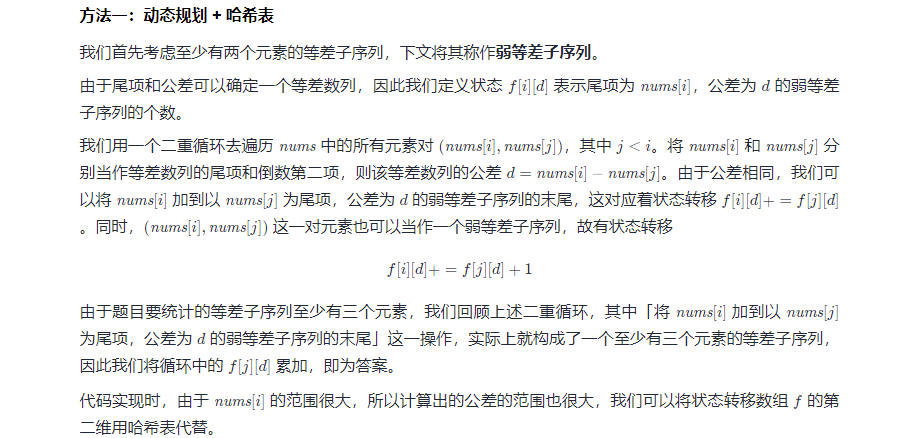
\includegraphics[width=.9\linewidth]{./pic/arithslice.png}

Define the type of the difference as Integer type instead of Long. This is because there is no valid arithmetic subsequence slice that can have difference out of the Integer value range. But we do need a long integer to filter out those invalid cases.

Preallocate the HashMap to avoid reallocation to deal with extreme cases.

Refrain from using lambda expressions inside loops.

\begin{minted}[frame=lines,fontsize=\scriptsize,linenos=false]{java}
public int numberOfArithmeticSlices(int [] arr) {
    int n = arr.length, ans = 0;
    Map<Integer, Integer> [] dp = new HashMap[n];
    dp[0] = new HashMap<>();
    for (int i = 1; i < n; i++) {
        dp[i] = new HashMap<>();
        for (int j = 0; j < i; j++) {
            long diff = (long)arr[i] - arr[j];
            if (diff > Integer.MAX_VALUE || diff < Integer.MIN_VALUE) continue;
            int dif = (int)diff;
            dp[i].put(dif, dp[i].getOrDefault(dif, 0) + 1);      // 这里先更新上
            if (dp[j].containsKey(dif)) {
                ans += dp[j].get(dif);    // 更新结果
                dp[i].put(dif, dp[i].get(dif) + dp[j].get(dif)); // 再加上之前累积的
            }
        }
    }
    return ans;
}
\end{minted}
% Emacs 27.1 (Org mode 8.2.7c)
\end{document}